\section{Estudos das deformações}
	
	\subsection{Considerações iniciais}
		\begin{itemize}
	\item Configuração do sólido: posição ocupada pelos pontos em um determinado instante $t$;
	\item Descrever a configuração deformada ($V$) a partir de uma configuração de referência ($V^r$);
	\item \sloppy Considerando um conjunto de pontos da Geometria Euclidiana ($E$), e seja, $(\vt{e}_1,\;\vt{e}_2,\;\vt{e}_3)$ uma base do espaço vetorial da geometria clássica.
\end{itemize}
	
Podemos definir $(0,\;\vt{e}_1,\;\vt{e}_2,\;\vt{e}_3)$ como um sistema de referência:

\begin{figure}[H]
	\centering
	\caption{Campo de deslocamentos.}
	

\tikzset{every picture/.style={line width=0.75pt}} %set default line width to 0.75pt        

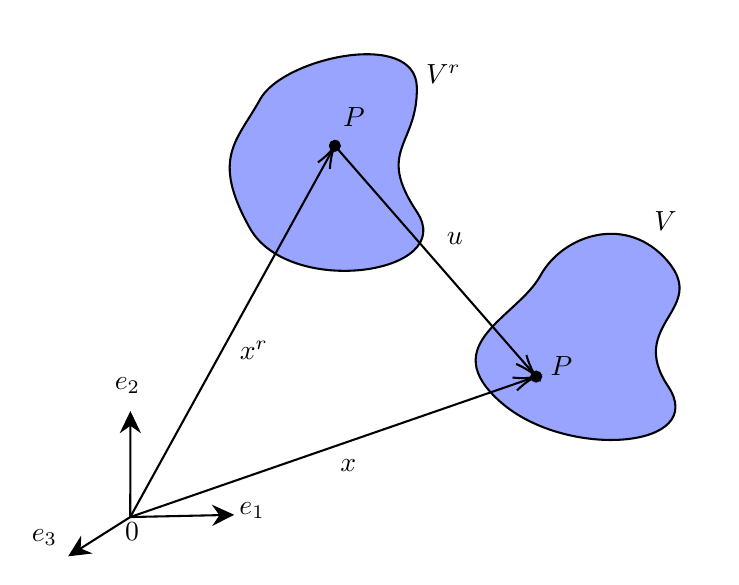
\begin{tikzpicture}[x=0.75pt,y=0.75pt,yscale=-1,xscale=1]
%uncomment if require: \path (0,264); %set diagram left start at 0, and has height of 264

%Shape: Polygon Curved [id:ds23301958927076183] 
\draw  [fill={rgb, 255:red, 0; green, 27; blue, 255 }  ,fill opacity=0.4 ] (132.5,31.7) .. controls (143.5,11.7) and (207.5,-2.3) .. (208,25.9) .. controls (208.5,54.1) and (188,55.9) .. (208,85.9) .. controls (228,115.9) and (146.5,127.7) .. (127.5,93.7) .. controls (108.5,59.7) and (121.5,51.7) .. (132.5,31.7) -- cycle ;
%Shape: Polygon Curved [id:ds07650390385014516] 
\draw  [fill={rgb, 255:red, 0; green, 27; blue, 255 }  ,fill opacity=0.4 ] (267.5,116.7) .. controls (278.5,96.7) and (309.5,86.7) .. (329,109.9) .. controls (348.5,133.1) and (309,139.9) .. (329,169.9) .. controls (349,199.9) and (280.5,205.7) .. (248.5,177.7) .. controls (216.5,149.7) and (256.5,136.7) .. (267.5,116.7) -- cycle ;
%Straight Lines [id:da5659027756383297] 
\draw    (69.92,232.98) -- (263.61,165.96) ;
\draw [shift={(265.5,165.3)}, rotate = 520.9100000000001] [color={rgb, 255:red, 0; green, 0; blue, 0 }  ][line width=0.75]    (10.93,-3.29) .. controls (6.95,-1.4) and (3.31,-0.3) .. (0,0) .. controls (3.31,0.3) and (6.95,1.4) .. (10.93,3.29)   ;
%Shape: Circle [id:dp33072264254260797] 
\draw  [fill={rgb, 255:red, 0; green, 0; blue, 0 }  ,fill opacity=1 ] (166.1,54.1) .. controls (166.1,52.78) and (167.17,51.7) .. (168.5,51.7) .. controls (169.83,51.7) and (170.9,52.78) .. (170.9,54.1) .. controls (170.9,55.43) and (169.83,56.5) .. (168.5,56.5) .. controls (167.17,56.5) and (166.1,55.43) .. (166.1,54.1) -- cycle ;
%Shape: Circle [id:dp6820829798134418] 
\draw  [fill={rgb, 255:red, 0; green, 0; blue, 0 }  ,fill opacity=1 ] (263.1,165.3) .. controls (263.1,163.98) and (264.17,162.9) .. (265.5,162.9) .. controls (266.83,162.9) and (267.9,163.98) .. (267.9,165.3) .. controls (267.9,166.63) and (266.83,167.7) .. (265.5,167.7) .. controls (264.17,167.7) and (263.1,166.63) .. (263.1,165.3) -- cycle ;
%Straight Lines [id:da5268734143852947] 
\draw    (69.92,232.98) -- (167.53,55.85) ;
\draw [shift={(168.5,54.1)}, rotate = 478.86] [color={rgb, 255:red, 0; green, 0; blue, 0 }  ][line width=0.75]    (10.93,-3.29) .. controls (6.95,-1.4) and (3.31,-0.3) .. (0,0) .. controls (3.31,0.3) and (6.95,1.4) .. (10.93,3.29)   ;
%Straight Lines [id:da4223642623796222] 
\draw    (168.5,54.1) -- (264.19,163.8) ;
\draw [shift={(265.5,165.3)}, rotate = 228.9] [color={rgb, 255:red, 0; green, 0; blue, 0 }  ][line width=0.75]    (10.93,-3.29) .. controls (6.95,-1.4) and (3.31,-0.3) .. (0,0) .. controls (3.31,0.3) and (6.95,1.4) .. (10.93,3.29)   ;
%Straight Lines [id:da15852304301408338] 
\draw    (69.92,232.98) -- (70,184.9) ;
\draw [shift={(70,181.9)}, rotate = 450.09] [fill={rgb, 255:red, 0; green, 0; blue, 0 }  ][line width=0.08]  [draw opacity=0] (10.72,-5.15) -- (0,0) -- (10.72,5.15) -- (7.12,0) -- cycle    ;
%Straight Lines [id:da35641451568895] 
\draw    (69.92,232.98) -- (117,231.97) ;
\draw [shift={(120,231.9)}, rotate = 538.76] [fill={rgb, 255:red, 0; green, 0; blue, 0 }  ][line width=0.08]  [draw opacity=0] (10.72,-5.15) -- (0,0) -- (10.72,5.15) -- (7.12,0) -- cycle    ;
%Straight Lines [id:da5944288129967534] 
\draw    (69.92,232.98) -- (42.54,250.3) ;
\draw [shift={(40,251.9)}, rotate = 327.69] [fill={rgb, 255:red, 0; green, 0; blue, 0 }  ][line width=0.08]  [draw opacity=0] (10.72,-5.15) -- (0,0) -- (10.72,5.15) -- (7.12,0) -- cycle    ;

% Text Node
\draw (121,224.3) node [anchor=north west][inner sep=0.75pt]    {$\vt{e}_{1}$};
% Text Node
\draw (169.71,203.74) node [anchor=north west][inner sep=0.75pt]    {$\vt{x}$};
% Text Node
\draw (121.21,146.94) node [anchor=north west][inner sep=0.75pt]    {$\vt{x}^{r}$};
% Text Node
\draw (211,13.3) node [anchor=north west][inner sep=0.75pt]    {$V^{r}$};
% Text Node
\draw (321,84.3) node [anchor=north west][inner sep=0.75pt]    {$V$};
% Text Node
\draw (61,164.3) node [anchor=north west][inner sep=0.75pt]    {$\vt{e}_{2}$};
% Text Node
\draw (21,237.3) node [anchor=north west][inner sep=0.75pt]    {$\vt{e}_{3}$};
% Text Node
\draw (271,154.3) node [anchor=north west][inner sep=0.75pt]    {$P$};
% Text Node
\draw (171,34.3) node [anchor=north west][inner sep=0.75pt]    {$P$};
% Text Node
\draw (221,94.3) node [anchor=north west][inner sep=0.75pt]    {$\vt{u}$};
% Text Node
\draw (66,234.3) node [anchor=north west][inner sep=0.75pt]    {$0$};


\end{tikzpicture}

\end{figure}
	
Os vetores dos pontos de referência ($\vt{x}^r$) e na configuração deformada ($\vt{x}$) em relação aos versores da base podem ser expressos na notação de Einstein:

\[\vt{x}^r=\vt{x}^r-\vt{0}=\sum_{i=1}^3x^{ri}e_i=x^{r1}\vt{e}_1+x^{r2}\vt{e}_2+x^{r3}\vt{e}_3\]
\[\vt{x}=\vt{x}-\vt{0}=\sum_{i=1}^3x^ie_i=x^1\vt{e}_1+x^2\vt{e}_2+x^3\vt{e}_3\]

Seja $f$ uma função que associa a posição de cada ponto na configuração $V^r$ a sua posição na configuração $V$. Tal aplicação é uma transformação de $V^r$ em $V$.
	
\[x^1=\hat{f}_1(x^{r1},\;x^{r2},\;x^{r3})\]
\[x^2=\hat{f}_2(x^{r1},\;x^{r2},\;x^{r3})\]
\[x^3=\hat{f}_3(x^{r1},\;x^{r2},\;x^{r3})\]

Aqui, o circunflexo denota \textit{em função de}, \textit{i.e.}, a coordenada $i$ da posição deformada está em função das coordenadas da posição de referência.
	
Exemplo: Considere um sólido cuja seção no plano $\vt{e}_1$, $\vt{e}_2$ é dado por:
	
//Inserir imagem
	
Caracterize os seguintes campos de deslocamento:
	
\begin{enumerate}[a)]
	\item Translação de corpo rígido de intensidade $\Delta$ na direção de $\vt{e}_1$;
	\item Rotação de corpo rígido em torno de $\vt{e}_3$ de intensidade $\varphi$.
\end{enumerate}
	
Resolução:
	
\begin{enumerate}[a)]
	\item
		\[
		\vt{u}=
			\begin{Bmatrix}
			u_1 \\ u_2 \\ u_3
			\end{Bmatrix}
			=
			\begin{Bmatrix}
				\Delta \\ 0 \\ 0
			\end{Bmatrix}
		\]
		\[\vt{u}=\vt{x}-\vt{x}^r
		\implies
		\vt{x}=
		\begin{cases} x^1=x^{r1}+u_1=x^{r1}+\Delta \\ x^2=x^{r2}+u_2=x^{r2} \\ x^3=x^{r3}+u_3=x^{r3}
		\end{cases}
		\]
	\item
		//Inserir imagem
			
		A configuração de referência:
		\[x^{r1}=r\cdot \cos\theta\]
		\[x^{r2}=r\cdot\sin\theta\]
		\[x^{r3}=0\;\text{(ou }x^{r3}\text{ para deixar genérico})\]
			
		A configuração deformada (a partir da imagem):
			
		\[u^1=r\cdot\cos(\varphi+\theta)-r\cdot\cos\theta\]
		\[u^1=r\cdot\cos\varphi\cdot\cos\theta-r\cdot\sin\varphi\cdot\sin\theta-r\cdot\cos\theta\]
			
		\[u^2=r\cdot\sin(\varphi+\theta)-r\cdot\sin\theta\]
		\[u^2=r\cdot\sin\varphi\cdot\cos\theta+r\cdot\sin\theta\cdot\cos\varphi-r\cdot\sin\theta\]
			
		Substituindo as coordenadas de referência nas coordenadas deformadas:

		\[u^1=x^{r1}\cdot\cos\varphi-x^{r2}\cdot\sin\varphi-x^{r1}\]
		\[u^2=x^{r1}\cdot\sin\varphi+x^{r2}\cdot\cos\varphi-x^{r2}\]
		\[u^3=0\]
			
		Como sabemos que $\vt{x}=\vt{x}^r+\utilde{\mathbf{u}}$, temos:
			
		\[
			\begin{cases}
				x^1=x^{r1}\cdot\cos\varphi-x^{r2}\cdot\sin\varphi \\ x^2=x^{r1}\cdot\sin\varphi+x^{r2}\cdot\cos\varphi \\ x^3=x^{r3}
			\end{cases}
		\]
			
		Podemos escrever também na forma matricial:
			
		\[
			\begin{Bmatrix}
				x^1 \\ x^2 \\ x^3
			\end{Bmatrix}
			=
			\begin{bmatrix}	
				\cos\varphi & -\sin\varphi & 0 \\
				\sin\varphi & \cos\varphi & 0 \\
				0 & 0 & 1
			\end{bmatrix}
			\begin{Bmatrix}
				x^{r1} \\ x^{r2} \\ x^{r3}
			\end{Bmatrix}							
		\]
\end{enumerate}
	
	\subsection{Deformação Normal e por Cisalhamento}
		\begin{figure}[H]
	\centering
	\caption{Deformação normal de uma fibra.}
	\vspace*{5mm}
	

\tikzset{every picture/.style={line width=0.75pt}} %set default line width to 0.75pt        

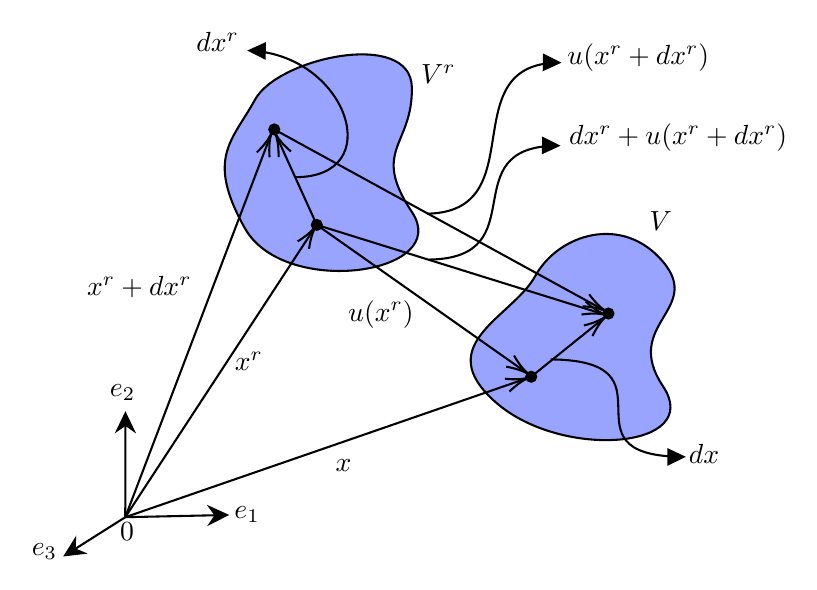
\begin{tikzpicture}[x=0.75pt,y=0.75pt,yscale=-1,xscale=1]
%uncomment if require: \path (0,292); %set diagram left start at 0, and has height of 292

%Shape: Polygon Curved [id:ds08619916045221121] 
\draw  [fill={rgb, 255:red, 0; green, 27; blue, 255 }  ,fill opacity=0.4 ] (427.5,132.8) .. controls (438.5,112.8) and (469.5,102.8) .. (489,126) .. controls (508.5,149.2) and (469,156) .. (489,186) .. controls (509,216) and (440.5,221.8) .. (408.5,193.8) .. controls (376.5,165.8) and (416.5,152.8) .. (427.5,132.8) -- cycle ;
%Shape: Polygon Curved [id:ds680978509087605] 
\draw  [fill={rgb, 255:red, 0; green, 27; blue, 255 }  ,fill opacity=0.4 ] (292.5,47.8) .. controls (303.5,27.8) and (367.5,13.8) .. (368,42) .. controls (368.5,70.2) and (348,72) .. (368,102) .. controls (388,132) and (306.5,143.8) .. (287.5,109.8) .. controls (268.5,75.8) and (281.5,67.8) .. (292.5,47.8) -- cycle ;
%Straight Lines [id:da27775957706905996] 
\draw    (322.2,108.25) -- (422.62,179.02) ;
\draw [shift={(424.26,180.17)}, rotate = 215.17000000000002] [color={rgb, 255:red, 0; green, 0; blue, 0 }  ][line width=0.75]    (10.93,-3.29) .. controls (6.95,-1.4) and (3.31,-0.3) .. (0,0) .. controls (3.31,0.3) and (6.95,1.4) .. (10.93,3.29)   ;
%Straight Lines [id:da02940601389234554] 
\draw    (322.2,108.25) -- (459.26,150.95) ;
\draw [shift={(461.17,151.54)}, rotate = 197.3] [color={rgb, 255:red, 0; green, 0; blue, 0 }  ][line width=0.75]    (10.93,-3.29) .. controls (6.95,-1.4) and (3.31,-0.3) .. (0,0) .. controls (3.31,0.3) and (6.95,1.4) .. (10.93,3.29)   ;
%Straight Lines [id:da04858175368526485] 
\draw    (229.92,249.08) -- (320.59,110.53) ;
\draw [shift={(321.69,108.86)}, rotate = 483.2] [color={rgb, 255:red, 0; green, 0; blue, 0 }  ][line width=0.75]    (10.93,-3.29) .. controls (6.95,-1.4) and (3.31,-0.3) .. (0,0) .. controls (3.31,0.3) and (6.95,1.4) .. (10.93,3.29)   ;
%Straight Lines [id:da3572803601625445] 
\draw    (229.92,249.08) -- (422.37,182.54) ;
\draw [shift={(424.26,181.89)}, rotate = 520.9300000000001] [color={rgb, 255:red, 0; green, 0; blue, 0 }  ][line width=0.75]    (10.93,-3.29) .. controls (6.95,-1.4) and (3.31,-0.3) .. (0,0) .. controls (3.31,0.3) and (6.95,1.4) .. (10.93,3.29)   ;
%Shape: Circle [id:dp7963034541993572] 
\draw  [fill={rgb, 255:red, 0; green, 0; blue, 0 }  ,fill opacity=1 ] (319.8,108.25) .. controls (319.8,106.92) and (320.87,105.85) .. (322.2,105.85) .. controls (323.53,105.85) and (324.6,106.92) .. (324.6,108.25) .. controls (324.6,109.58) and (323.53,110.65) .. (322.2,110.65) .. controls (320.87,110.65) and (319.8,109.58) .. (319.8,108.25) -- cycle ;
%Shape: Circle [id:dp5549951934814357] 
\draw  [fill={rgb, 255:red, 0; green, 0; blue, 0 }  ,fill opacity=1 ] (423.1,181.4) .. controls (423.1,180.07) and (424.17,179) .. (425.5,179) .. controls (426.83,179) and (427.9,180.07) .. (427.9,181.4) .. controls (427.9,182.73) and (426.83,183.8) .. (425.5,183.8) .. controls (424.17,183.8) and (423.1,182.73) .. (423.1,181.4) -- cycle ;
%Straight Lines [id:da09097339056268305] 
\draw    (229.92,249.08) -- (230,201) ;
\draw [shift={(230,198)}, rotate = 450.09] [fill={rgb, 255:red, 0; green, 0; blue, 0 }  ][line width=0.08]  [draw opacity=0] (10.72,-5.15) -- (0,0) -- (10.72,5.15) -- (7.12,0) -- cycle    ;
%Straight Lines [id:da3893826545167065] 
\draw    (229.92,249.08) -- (277,248.06) ;
\draw [shift={(280,248)}, rotate = 538.76] [fill={rgb, 255:red, 0; green, 0; blue, 0 }  ][line width=0.08]  [draw opacity=0] (10.72,-5.15) -- (0,0) -- (10.72,5.15) -- (7.12,0) -- cycle    ;
%Straight Lines [id:da21469655729558346] 
\draw    (229.92,249.08) -- (202.54,266.4) ;
\draw [shift={(200,268)}, rotate = 327.69] [fill={rgb, 255:red, 0; green, 0; blue, 0 }  ][line width=0.08]  [draw opacity=0] (10.72,-5.15) -- (0,0) -- (10.72,5.15) -- (7.12,0) -- cycle    ;
%Straight Lines [id:da4866033538311314] 
\draw    (425.5,181.4) -- (459.9,153.66) ;
\draw [shift={(461.46,152.4)}, rotate = 501.11] [color={rgb, 255:red, 0; green, 0; blue, 0 }  ][line width=0.75]    (10.93,-3.29) .. controls (6.95,-1.4) and (3.31,-0.3) .. (0,0) .. controls (3.31,0.3) and (6.95,1.4) .. (10.93,3.29)   ;
%Curve Lines [id:da9181705698289111] 
\draw    (434.9,173.05) .. controls (497.94,173.71) and (437.92,218.91) .. (497.21,219.98) ;
\draw [shift={(500,220)}, rotate = 539.73] [fill={rgb, 255:red, 0; green, 0; blue, 0 }  ][line width=0.08]  [draw opacity=0] (8.93,-4.29) -- (0,0) -- (8.93,4.29) -- cycle    ;
%Straight Lines [id:da8085286493536537] 
\draw    (322.2,108.25) -- (303.08,66.11) ;
\draw [shift={(302.26,64.29)}, rotate = 425.6] [color={rgb, 255:red, 0; green, 0; blue, 0 }  ][line width=0.75]    (10.93,-3.29) .. controls (6.95,-1.4) and (3.31,-0.3) .. (0,0) .. controls (3.31,0.3) and (6.95,1.4) .. (10.93,3.29)   ;
%Straight Lines [id:da06391364265309418] 
\draw    (301.7,62.25) -- (459.7,148.87) ;
\draw [shift={(461.46,149.83)}, rotate = 208.73] [color={rgb, 255:red, 0; green, 0; blue, 0 }  ][line width=0.75]    (10.93,-3.29) .. controls (6.95,-1.4) and (3.31,-0.3) .. (0,0) .. controls (3.31,0.3) and (6.95,1.4) .. (10.93,3.29)   ;
%Curve Lines [id:da6195997993819029] 
\draw [color={rgb, 255:red, 0; green, 0; blue, 0 }  ,draw opacity=1 ]   (311.95,85.25) .. controls (356.05,85.25) and (337.48,27.63) .. (291.55,24.38) ;
\draw [shift={(288.7,24.25)}, rotate = 361.19] [fill={rgb, 255:red, 0; green, 0; blue, 0 }  ,fill opacity=1 ][line width=0.08]  [draw opacity=0] (8.93,-4.29) -- (0,0) -- (8.93,4.29) -- cycle    ;
%Curve Lines [id:da8347033822514986] 
\draw    (375.2,102.85) .. controls (427.05,102.09) and (387.51,31.48) .. (437.68,30.09) ;
\draw [shift={(440.04,30.08)}, rotate = 180.82] [fill={rgb, 255:red, 0; green, 0; blue, 0 }  ][line width=0.08]  [draw opacity=0] (8.93,-4.29) -- (0,0) -- (8.93,4.29) -- cycle    ;
%Curve Lines [id:da7704708098624058] 
\draw    (376.36,124.96) .. controls (428.21,124.2) and (387.15,70.95) .. (437.29,70.08) ;
\draw [shift={(439.64,70.08)}, rotate = 180.82] [fill={rgb, 255:red, 0; green, 0; blue, 0 }  ][line width=0.08]  [draw opacity=0] (8.93,-4.29) -- (0,0) -- (8.93,4.29) -- cycle    ;
%Straight Lines [id:da08511227281768252] 
\draw    (229.92,249.08) -- (299.55,66.15) ;
\draw [shift={(300.26,64.29)}, rotate = 470.84] [color={rgb, 255:red, 0; green, 0; blue, 0 }  ][line width=0.75]    (10.93,-3.29) .. controls (6.95,-1.4) and (3.31,-0.3) .. (0,0) .. controls (3.31,0.3) and (6.95,1.4) .. (10.93,3.29)   ;
%Shape: Circle [id:dp47512159867268555] 
\draw  [fill={rgb, 255:red, 0; green, 0; blue, 0 }  ,fill opacity=1 ] (299.3,62.25) .. controls (299.3,60.92) and (300.37,59.85) .. (301.7,59.85) .. controls (303.03,59.85) and (304.1,60.92) .. (304.1,62.25) .. controls (304.1,63.58) and (303.03,64.65) .. (301.7,64.65) .. controls (300.37,64.65) and (299.3,63.58) .. (299.3,62.25) -- cycle ;
%Shape: Circle [id:dp20685874584691932] 
\draw  [fill={rgb, 255:red, 0; green, 0; blue, 0 }  ,fill opacity=1 ] (460.3,150.95) .. controls (460.3,149.62) and (461.37,148.55) .. (462.7,148.55) .. controls (464.03,148.55) and (465.1,149.62) .. (465.1,150.95) .. controls (465.1,152.28) and (464.03,153.35) .. (462.7,153.35) .. controls (461.37,153.35) and (460.3,152.28) .. (460.3,150.95) -- cycle ;

% Text Node
\draw (281,242.4) node [anchor=north west][inner sep=0.75pt]    {$\vt{e}_{1}$};
% Text Node
\draw (329.71,219.64) node [anchor=north west][inner sep=0.75pt]    {$\vt{x}$};
% Text Node
\draw (281.21,168.04) node [anchor=north west][inner sep=0.75pt]    {$\vt{x}^{r}$};
% Text Node
\draw (371,29.4) node [anchor=north west][inner sep=0.75pt]    {$V^{r}$};
% Text Node
\draw (481,100.4) node [anchor=north west][inner sep=0.75pt]    {$V$};
% Text Node
\draw (221,183.6) node [anchor=north west][inner sep=0.75pt]    {$\vt{e}_{2}$};
% Text Node
\draw (183.4,260.2) node [anchor=north west][inner sep=0.75pt]    {$\vt{e}_{3}$};
% Text Node
\draw (335.83,143.07) node [anchor=north west][inner sep=0.75pt]    {$\vt{u}(\vt{x}^r)$};
% Text Node
\draw (226,250.4) node [anchor=north west][inner sep=0.75pt]    {$0$};
% Text Node
\draw (500,212.4) node [anchor=north west][inner sep=0.75pt]    {$d\vt{x}$};
% Text Node
\draw (262.67,13.73) node [anchor=north west][inner sep=0.75pt]    {$d\vt{x}^{r}$};
% Text Node
\draw (441.47,19.53) node [anchor=north west][inner sep=0.75pt]    {$\vt{u}(\vt{x}^{r} +d\vt{x}^{r})$};
% Text Node
\draw (442.27,57.93) node [anchor=north west][inner sep=0.75pt]    {$d\vt{x}^{r}+\vt{u}(\vt{x}^{r} +d\vt{x}^{r})$};
% Text Node
\draw (210.07,131.53) node [anchor=north west][inner sep=0.75pt]    {$\vt{x}^{r} +d\vt{x}^{r}$};

\end{tikzpicture}

\end{figure}

O assunto agora são fibras; como as fibras sofrem deformação. Seja $d\vt{x}^r$ o vetor infinitesimal que representa uma fibra a partir do ponto $\vt{x}^r$; $d\vt{x}$ o vetor infinitesimal da mesma fibra agora na configuração deformada, partindo do ponto $\vt{x}$.
Para que o vetor $d\vt{x}^r$ deforme e se transforme em $d\vt{x}$, deve ocorrer uma transformação que depende de $\vt{x}^r+d\vt{x}^r$, \textit{i.e.}, uma transformação $\vt{u}(\vt{x}^r+d\vt{x}^r)$.

Algumas relações podem ser estabelecidas a partir da imagem acima, sendo:
\[\vt{u}(\vt{x}^r)=d\vt{x}^r+\vt{u}(\vt{x}^r+d\vt{x}^r)\]

E a fibra na configuração deformada:	
\[d\vt{x}=d\vt{x}^r+\vt{u}(\vt{x}^r+d\vt{x}^r)-\vt{u}(\vt{x}^r)\]

A equação acima na forma de componentes:
\[dx^i=dx^{ri}+u^i(x^{r1}+dx^{r1},\;x^{r2}+dx^{r2},\;x^{r3}+dx^{r3})-u^i(x^{r1},\;x^{r2},\;x^{r3})\]

Lembrando de cálculo com múltiplas variáveis:
\[u^i(x^{r1}+dx^{r1},\;x^{r2}+dx^{r2},\;x^{r3}+dx^{r3})-u^i(x^{r1},\;x^{r2},\;x^{r3})=\frac{\partial u^i}{\partial x^{r1}}dx^{r1}+\frac{\partial u^i}{\partial x^{r2}}dx^{r2}+\frac{\partial u^i}{\partial x^{r3}}dx^{r3}\]

Para $i=1,\;2$ e $3$. Essa iteração diz que cada coordenada $i$ depende de acontecimentos nas $3$ dimensões do espaço euclidiano.

Reescrevendo na forma matricial:
\[
	\underbrace{
	\begin{Bmatrix}
		dx^1 \\ dx^2 \\ dx^3
	\end{Bmatrix}
	}_{\displaystyle d\vt{x}}
	=
	\underbrace{
	\begin{Bmatrix}
		dx^{r1} \\ dx^{r2} \\ dx^{r3}
	\end{Bmatrix}
	}_{\displaystyle d\vt{x}^r}
	+
	\underbrace{
	\begin{bmatrix}
		\frac{\partial u^1}{\partial x^{r1}} & \frac{\partial u^1}{\partial x^{r2}} & \frac{\partial u^1}{\partial x^{r3}} \\
		\frac{\partial u^2}{\partial x^{r1}} & \frac{\partial u^2}{\partial x^{r2}} & \frac{\partial u^2}{\partial x^{r3}} \\
		\frac{\partial u^3}{\partial x^{r1}} & \frac{\partial u^3}{\partial x^{r2}} & \frac{\partial u^3}{\partial x^{r3}}
	\end{bmatrix}
	}_{\displaystyle\nabla\vt{u}=\ts{L}}
	\underbrace{
	\begin{Bmatrix}
		dx^{r1} \\ dx^{r2} \\ dx^{r3}
	\end{Bmatrix}
	}_{\displaystyle d\vt{x}^r}
\]

Onde $\nabla\vt{u}$ é o \textbf{gradiente dos deslocamentos}.

Logo,
\[d\vt{x}=d\vt{x}^r+\nabla\vt{u}\;d\vt{x}^r\]

Colocando $d\vt{x}^r$ em evidência, temos:
\[d\vt{x}=\underbrace{(\ts{I}+\nabla\vt{u})}_{\displaystyle \ts{F}}d\vt{x}^r\]

Onde $\ts{F}$ é o \textbf{gradiente das deformações}.

Portanto, temos:
\begin{equation}
	d\vt{x}=\ts{F}\;d\vt{x}^r
\end{equation}

Ou seja, a fibra deformada agora pode ser obtida a partir do gradiente dos deslocamentos ($\nabla\vt{u}$) e também a partir do gradiente das deformações ($\ts{F}$).

O gradiente das deformações pode ser reescrito como:
\[
	\ts{F}=
	\begin{bmatrix}
		1+\frac{\partial u^1}{\partial x^{r1}} & \frac{\partial u^1}{\partial x^{r2}} & \frac{\partial u^1}{\partial x^{r3}} \\
		\frac{\partial u^2}{\partial x^{r1}} & 1+\frac{\partial u^2}{\partial x^{r2}} & \frac{\partial u^2}{\partial x^{r3}} \\
		\frac{\partial u^3}{\partial x^{r1}} & \frac{\partial u^3}{\partial x^{r2}} & 1+\frac{\partial u^3}{\partial x^{r3}}
	\end{bmatrix}
\]

Ou ainda, usando notação indicial de Einstein:
\[F_{ij}=\nabla u_{ij}+\delta_{ij}\]

Onde $\delta_{ij}$ é o delta de Kronecker, \textit{i.e.}: $\delta_{ij}=\begin{cases} 1, & \text{se } i=j \\ 0, & \text{se } i\neq j \end{cases}$

E em notação indicial, temos:
\[\nabla u_{ij}=\frac{\partial u^i}{\partial x^{rj}}\]

Agora, expressemos:
\[\vt{u}=\vt{x}-\vt{x}^r\implies \vt{x}=\vt{u}+\vt{x}^r\]
\[x^i=u^i+x^{ri}\]

Derivando ambos os lados da notação indicial acima em relação a $\vt{x}^r$, temos:
\[\underbrace{\frac{\partial x^i}{\partial x^{rj}}}_{\displaystyle\ts{F}}=\underbrace{\frac{\partial u^i}{\partial x^{rj}}}_{\displaystyle\nabla u_{ij}}+\underbrace{\frac{\partial x^{ri}}{\partial x^{rj}}}_{\displaystyle\delta_{ij}}\]

Ou seja, agora o gradiente das deformações está em função da transformação e sua forma matricial é:
\[
	\ts{F}=
	\begin{bmatrix}
		\frac{\partial x^1}{\partial x^{r1}} & \frac{\partial x^1}{\partial x^{r2}} & \frac{\partial x^1}{\partial x^{r3}} \\
		\frac{\partial x^2}{\partial x^{r1}} & \frac{\partial x^2}{\partial x^{r2}} & \frac{\partial x^2}{\partial x^{r3}} \\
		\frac{\partial x^3}{\partial x^{r1}} & \frac{\partial x^3}{\partial x^{r2}} & \frac{\partial x^3}{\partial x^{r3}}
	\end{bmatrix}
\]

Lembrete sobre operadores lineares:

$\ts{F}$ e $\nabla\vt{u}$  são operadores lineares de $E\rightarrow E$. Seja $\ts{T}$ um operador linear:
\[\ts{T}(\alpha\vt{x}+\beta\vt{y})=\alpha\ts{T}\vt{x}+\beta\ts{T}\vt{y},\;\forall\;\vt{x}\text{ e }\vt{y}\in\text{$E$}\]

//Inserir imagem

\[
	\begin{Bmatrix}
		b_1 \\ b_2 \\ b_3
	\end{Bmatrix}
	=
	\underbrace{
	\begin{bmatrix}
		T_{11} & T_{12} & T_{13} \\
		T_{21} & T_{22} & T_{23} \\
		T_{31} & T_{32} & T_{33}
	\end{bmatrix}
	}_{\displaystyle\ts{T}}
	\begin{Bmatrix}
		a_1 \\ a_2 \\ a_3
	\end{Bmatrix}
\]

Obs: Para o curso, um operador linear tem a mesma função de um tensor (simplificando).
	
	\subsection{Tensor das Deformações de Green-Lagrange}
		//Inserir imagem
	
Onde $\hat{\utilde{\mathbf{m}}}^r$ é um versor, $\displaystyle\frac{d\utilde{\mathbf{x}}^r}{||d\utilde{\mathbf{x}}^r||}=1$, $ds^r$ é o comprimento infinitesimal de uma fibra na configuração de referência na direção de $\hat{\utilde{\mathbf{m}}}^r$ e $ds$ é o comprimento dessa mesma fibra na configuração deformada. Os comprimentos são definidos como:
\[ds^r=||d\utilde{\mathbf{x}}^r||=(d\utilde{\mathbf{x}}^r\cdot d\utilde{\mathbf{x}}^r)^{\frac{1}{2}}\]
\[ds=||d\utilde{\mathbf{x}}||=(d\utilde{\mathbf{x}}\cdot d\utilde{\mathbf{x}})^{\frac{1}{2}}\]
	
Lembrando sobre operadores lineares: Seja $\underline{\mathbf{A}}$ um operador linear ou tensor, temos
\[\utilde{\mathbf{a}}\cdot\underline{\mathbf{A}}\utilde{\mathbf{b}}=\utilde{\mathbf{b}}\cdot\underline{\mathbf{A}}^{\text{T}}\utilde{\mathbf{a}},\;\forall\;\mathbf{\utilde{\mathbf{a}}}\text{ e }\mathbf{\utilde{\mathbf{b}}}\in\text{$E$}\]
	
Quando $\underline{\mathbf{A}}=\underline{\mathbf{A}}^{\text{T}}$, $\underline{\mathbf{A}}$ é simétrico.
	
\textbf{Exemplo}: A \textit{interpolação quadrática} ou \textit{alongamento quadrático} é definida como:
\[\varepsilon_q=\frac{1}{2}\frac{(ds)^2-(ds^r)^2}{(ds^r)^2}\]
	
Sabendo que,
\[ds^2=d\utilde{\mathbf{x}}\cdot d\utilde{\mathbf{x}}=\underbrace{\underline{\mathbf{F}}d\utilde{\mathbf{x}}^r}_{\displaystyle\utilde{\mathbf{v}}}\cdot\underline{\mathbf{F}}d\utilde{\mathbf{x}}^r\]
\[ds^2=\utilde{\mathbf{v}}\cdot\underline{\mathbf{F}}d\utilde{\mathbf{x}}^r\]
\[ds^2=d\utilde{\mathbf{x}}^r\cdot\underline{\mathbf{F}}^{\text{T}}\utilde{\mathbf{v}}\]
\[ds^2=d\utilde{\mathbf{x}}^r\cdot\underline{\mathbf{F}}^{\text{T}}\underline{\mathbf{F}}d\utilde{\mathbf{x}}^r\]
	
Logo,
\[\varepsilon_q=\frac{1}{2}\frac{(d\utilde{\mathbf{x}}^r\cdot\underline{\mathbf{F}}^{\text{T}}\underline{\mathbf{F}}d\utilde{\mathbf{x}}^r)-(d\utilde{\mathbf{x}}^r\cdot d\utilde{\mathbf{x}}^r)}{d\utilde{\mathbf{x}}^r\cdot d\utilde{\mathbf{x}}^r}\]
	
Lembrando que,
\[d\utilde{\mathbf{x}}^r=||d\utilde{\mathbf{x}}^r||\hat{\utilde{\mathbf{m}}}^r=ds^r\hat{\utilde{\mathbf{m}}}^r\]
	
Então,
\[\varepsilon_q=\frac{1}{2}\frac{(ds^r\hat{\utilde{\mathbf{m}}}^r\cdot\underline{\mathbf{F}}^{\text{T}}\underline{\mathbf{F}}d\utilde{\mathbf{x}}^r)-(ds^r\hat{\utilde{\mathbf{m}}}^r\cdot ds^r\hat{\utilde{\mathbf{m}}}^r)}{ds^r\hat{\utilde{\mathbf{m}}}^r\cdot ds^r\hat{\utilde{\mathbf{m}}}^r}\]
\[\varepsilon_q=\frac{1}{2}\frac{ds^r\hat{\utilde{\mathbf{m}}}^r\cdot(\underline{\mathbf{F}}^{\text{T}}\underline{\mathbf{F}}-\underline{\mathbf{I}})ds^r\hat{\utilde{\mathbf{m}}}^r}{ds^r\hat{\utilde{\mathbf{m}}}^r\cdot ds^r\hat{\utilde{\mathbf{m}}}^r}\]
\[\varepsilon_q=\frac{1}{2}[\hat{\utilde{\mathbf{m}}}^r\cdot(\underline{\mathbf{F}}^{\text{T}}\underline{\mathbf{F}}-\underline{\mathbf{I}})\hat{\utilde{\mathbf{m}}}^r]\]
\[\varepsilon_q=\hat{\utilde{\mathbf{m}}}^r\cdot\underbrace{\frac{1}{2}(\underline{\mathbf{F}}^{\text{T}}\underline{\mathbf{F}}-\underline{\mathbf{I}})}_{\displaystyle\underline{\mathbf{E}}}\hat{\utilde{\mathbf{m}}}^r\]
	
\[\underline{\mathbf{E}}=\frac{1}{2}(\underline{\mathbf{F}}^{\text{T}}\underline{\mathbf{F}}-\underline{\mathbf{I}})\]
\[\varepsilon_q(\hat{\utilde{\mathbf{m}}}^r)=\hat{\utilde{\mathbf{m}}}^r\cdot\underline{\mathbf{E}}\hat{\utilde{\mathbf{m}}}^r\]
	
Onde $\underline{\mathbf{E}}$ é o Tensor das Deformações de Green-Lagrange e vale para qualquer magnitude de deslocamento. Algumas literaturas chamam de \textit{finite displacement} os deslocamentos de qualquer magnitude.
	
Agora na notação de Einstein:
\[E_{ij}=\frac{1}{2}\left(\frac{\partial x^k}{\partial x^{ri}}\frac{\partial x^k}{\partial x^{rj}}-\delta_{ij}\right)\]
	
Expressando os componentes de $\underline{\mathbf{E}}$ a partir do campo de deslocamentos:
\[\underline{\mathbf{E}}=\frac{1}{2}[(\nabla\utilde{\mathbf{u}}^{\text{T}}+\underline{\mathbf{I}})(\nabla\utilde{\mathbf{u}}+\underline{\mathbf{I}})-\underline{\mathbf{I}}]\]
\[\underline{\mathbf{E}}=\frac{1}{2}(\nabla\utilde{\mathbf{u}}^{\text{T}}\nabla\utilde{\mathbf{u}}+\nabla\utilde{\mathbf{u}}^{\text{T}}+\nabla\utilde{\mathbf{u}}+\underline{\mathbf{I}}-\underline{\mathbf{I}})\]
\[\underline{\mathbf{E}}=\frac{1}{2}(\nabla\utilde{\mathbf{u}}+\nabla\utilde{\mathbf{u}}^{\text{T}}+\nabla\utilde{\mathbf{u}}^{\text{T}}\nabla\utilde{\mathbf{u}})\]
	
Na notação de Einstein:
\[E_{ij}=\frac{1}{2}\left(\frac{\partial u^i}{\partial x^{rj}}+\frac{\partial u^j}{\partial x^{ri}}+\underbrace{\frac{\partial u^k}{\partial x^{ri}}\frac{\partial u^k}{\partial x^{rj}}}_{*}\right)\]
	
Sendo $*$:
\[\frac{\partial u^k}{\partial x^{ri}}\frac{\partial u^k}{\partial x^{rj}}=\frac{\partial u^1}{\partial x^{ri}}\frac{\partial u^1}{\partial x^{rj}}+\frac{\partial u^2}{\partial x^{ri}}\frac{\partial u^2}{\partial x^{rj}}+\frac{\partial u^3}{\partial x^{ri}}\frac{\partial u^3}{\partial x^{rj}}\]
	
Acima, $E_{ij}$ denota equações de compatibilidade; uma relação deslocamentos-deformações.
	
	\subsection{Medidas de deformação/alongamento}
		\begin{itemize}
	\item Estiramento ou \textit{stretch}:
		\[\lambda=\frac{ds}{ds^r}\]
	\item Alongamento linear:
		\[\varepsilon_l=\frac{ds-ds^r}{ds^r}\]
	\item Alongamento quadrático:
		\[\varepsilon_q=\frac{1}{2}\frac{(ds)^2-(ds^r)^2}{(ds^r)^2}=\frac{1}{2}\left[\left(\frac{ds}{ds^r}\right)^2-1\right]=\frac{1}{2}(\lambda^2-1)\]
	\item Alongamento logarítmico ou de Henry:
		\[\varepsilon_n=\ln \left(\frac{ds}{ds^r}\right)\]
	\item Alongamento hiperbólico ou de Reiner:
		\[\varepsilon_h=\frac{ds^r}{ds}\]
	\item Alongamento hiperbólico quadrático ou de Almansi:
		\[\varepsilon_{hq}=\frac{1}{2}\frac{(ds^r)^2-(ds)^2}{(ds)^2}\]
\end{itemize}

		\subsubsection{Relação entre alongamentos quadráticos e lineares}
			Para o alongamento quadrático:
\[\varepsilon_q=\frac{1}{2}(\lambda^2-1)\]
\[\lambda^2=1+2\varepsilon_q\]
\[\lambda=\sqrt{1+2\varepsilon_q}\]
\[\lambda(\hat{\utilde{\mathbf{m}}}^r)=\sqrt{1+2(\hat{\utilde{\mathbf{m}}}^r\cdot\underline{\mathbf{E}}\hat{\utilde{\mathbf{m}}}^r)}\]

Para o alongamento linear:
\[\varepsilon_l=\lambda-1\]
\[\varepsilon_l(\hat{\utilde{\mathbf{m}}}^r)=\sqrt{1+2(\hat{\utilde{\mathbf{m}}}^r\cdot\underline{\mathbf{E}}\hat{\utilde{\mathbf{m}}}^r)}-1\]
\[\varepsilon_l(\hat{\utilde{\mathbf{m}}}^r)=\sqrt{1+2\varepsilon_q}-1\]
	
	\subsection{Variação do ângulo entre fibras (distorção)}
		\begin{figure}[H]
	\centering
	\caption{Variação do ângulo entre fibras inicialmente ortogonais.}
	\vspace*{5mm}
	

\tikzset{every picture/.style={line width=0.75pt}} %set default line width to 0.75pt        

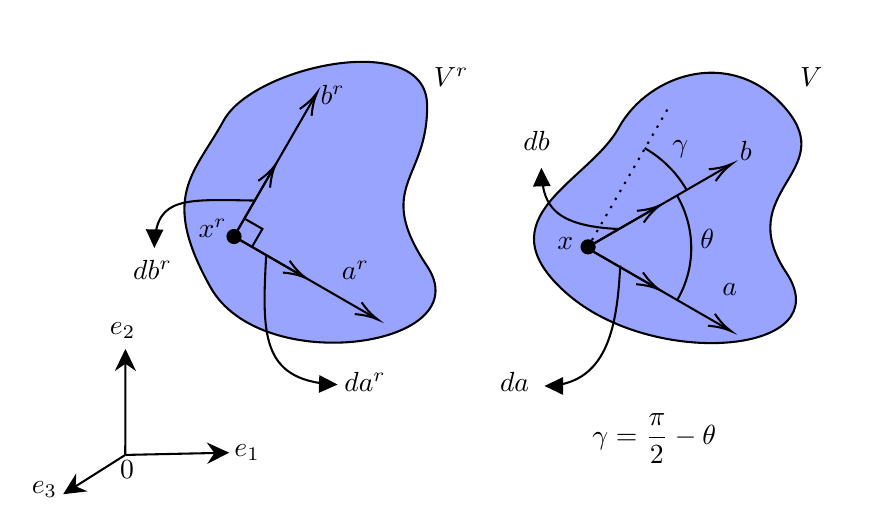
\begin{tikzpicture}[x=0.75pt,y=0.75pt,yscale=-1,xscale=1]
%uncomment if require: \path (0,249); %set diagram left start at 0, and has height of 249

%Shape: Polygon Curved [id:ds37090510589079506] 
\draw  [fill={rgb, 255:red, 0; green, 27; blue, 255 }  ,fill opacity=0.4 ] (443.7,47.62) .. controls (458.13,21.39) and (498.78,8.28) .. (524.35,38.7) .. controls (549.92,69.12) and (498.12,78.04) .. (524.35,117.38) .. controls (550.58,156.72) and (460.75,164.32) .. (418.79,127.61) .. controls (376.83,90.89) and (429.28,73.84) .. (443.7,47.62) -- cycle ;
%Shape: Regular Polygon [id:dp5727859442047756] 
\draw  [fill={rgb, 255:red, 0; green, 27; blue, 255 }  ,fill opacity=0.4 ] (253.42,44.02) .. controls (267.69,18.08) and (350.69,-0.07) .. (351.33,36.5) .. controls (351.98,73.07) and (325.4,75.4) .. (351.33,114.31) .. controls (377.27,153.21) and (271.58,168.52) .. (246.94,124.42) .. controls (222.3,80.33) and (239.16,69.96) .. (253.42,44.02) -- cycle ;
%Straight Lines [id:da34741946249595057] 
\draw    (205.92,205.28) -- (206,157.2) ;
\draw [shift={(206,154.2)}, rotate = 450.09] [fill={rgb, 255:red, 0; green, 0; blue, 0 }  ][line width=0.08]  [draw opacity=0] (10.72,-5.15) -- (0,0) -- (10.72,5.15) -- (7.12,0) -- cycle    ;
%Straight Lines [id:da35183475808822884] 
\draw    (205.92,205.28) -- (253,204.26) ;
\draw [shift={(256,204.2)}, rotate = 538.76] [fill={rgb, 255:red, 0; green, 0; blue, 0 }  ][line width=0.08]  [draw opacity=0] (10.72,-5.15) -- (0,0) -- (10.72,5.15) -- (7.12,0) -- cycle    ;
%Straight Lines [id:da3444772189505243] 
\draw    (205.92,205.28) -- (178.54,222.6) ;
\draw [shift={(176,224.2)}, rotate = 327.69] [fill={rgb, 255:red, 0; green, 0; blue, 0 }  ][line width=0.08]  [draw opacity=0] (10.72,-5.15) -- (0,0) -- (10.72,5.15) -- (7.12,0) -- cycle    ;
%Shape: Ellipse [id:dp7016292540356281] 
\draw  [fill={rgb, 255:red, 0; green, 0; blue, 0 }  ,fill opacity=1 ] (426.03,103.73) .. controls (426.75,102.14) and (428.61,101.44) .. (430.2,102.16) .. controls (431.78,102.88) and (432.48,104.74) .. (431.76,106.33) .. controls (431.05,107.91) and (429.18,108.61) .. (427.6,107.89) .. controls (426.01,107.18) and (425.31,105.31) .. (426.03,103.73) -- cycle ;
%Curve Lines [id:da9364210310002001] 
\draw    (443.9,96.45) .. controls (412.41,95.04) and (407.35,84.85) .. (406.51,69.88) ;
\draw [shift={(406.4,66.95)}, rotate = 448.57] [fill={rgb, 255:red, 0; green, 0; blue, 0 }  ][line width=0.08]  [draw opacity=0] (8.93,-4.29) -- (0,0) -- (8.93,4.29) -- cycle    ;
%Straight Lines [id:da07400897737098244] 
\draw    (258.32,100.05) -- (297.32,32.5) ;
\draw [shift={(298.32,30.77)}, rotate = 480] [color={rgb, 255:red, 0; green, 0; blue, 0 }  ][line width=0.75]    (10.93,-3.29) .. controls (6.95,-1.4) and (3.31,-0.3) .. (0,0) .. controls (3.31,0.3) and (6.95,1.4) .. (10.93,3.29)   ;
%Straight Lines [id:da013971101698424304] 
\draw    (258.32,100.05) -- (325.87,139.05) ;
\draw [shift={(327.6,140.05)}, rotate = 210] [color={rgb, 255:red, 0; green, 0; blue, 0 }  ][line width=0.75]    (10.93,-3.29) .. controls (6.95,-1.4) and (3.31,-0.3) .. (0,0) .. controls (3.31,0.3) and (6.95,1.4) .. (10.93,3.29)   ;
%Straight Lines [id:da3279167723732044] 
\draw    (258.32,100.05) -- (291.23,119.05) ;
\draw [shift={(292.96,120.05)}, rotate = 210] [color={rgb, 255:red, 0; green, 0; blue, 0 }  ][line width=0.75]    (10.93,-3.29) .. controls (6.95,-1.4) and (3.31,-0.3) .. (0,0) .. controls (3.31,0.3) and (6.95,1.4) .. (10.93,3.29)   ;
%Straight Lines [id:da2868069526989574] 
\draw    (258.32,100.05) -- (277.32,67.14) ;
\draw [shift={(278.32,65.41)}, rotate = 480] [color={rgb, 255:red, 0; green, 0; blue, 0 }  ][line width=0.75]    (10.93,-3.29) .. controls (6.95,-1.4) and (3.31,-0.3) .. (0,0) .. controls (3.31,0.3) and (6.95,1.4) .. (10.93,3.29)   ;
%Shape: Right Angle [id:dp3447995497166503] 
\draw   (263.32,91.39) -- (271.98,96.39) -- (266.98,105.05) ;

%Curve Lines [id:da20063713589439125] 
\draw    (273.8,108.98) .. controls (271.85,146.42) and (271.04,169.03) .. (305.48,171.25) ;
\draw [shift={(308.2,171.38)}, rotate = 181.85] [fill={rgb, 255:red, 0; green, 0; blue, 0 }  ][line width=0.08]  [draw opacity=0] (8.93,-4.29) -- (0,0) -- (8.93,4.29) -- cycle    ;
%Shape: Ellipse [id:dp9761978258289457] 
\draw  [fill={rgb, 255:red, 0; green, 0; blue, 0 }  ,fill opacity=1 ] (255.47,98.71) .. controls (256.21,97.14) and (258.09,96.46) .. (259.66,97.2) .. controls (261.23,97.94) and (261.91,99.82) .. (261.17,101.39) .. controls (260.43,102.96) and (258.55,103.64) .. (256.98,102.9) .. controls (255.4,102.16) and (254.73,100.28) .. (255.47,98.71) -- cycle ;
%Curve Lines [id:da9063509801222673] 
\draw    (268.32,82.73) .. controls (234.32,82.08) and (221.44,81.13) .. (220.02,102.73) ;
\draw [shift={(219.9,105.55)}, rotate = 271.17] [fill={rgb, 255:red, 0; green, 0; blue, 0 }  ][line width=0.08]  [draw opacity=0] (8.93,-4.29) -- (0,0) -- (8.93,4.29) -- cycle    ;
%Straight Lines [id:da4322790233128786] 
\draw    (428.9,105.03) -- (496.45,66.03) ;
\draw [shift={(498.18,65.03)}, rotate = 510] [color={rgb, 255:red, 0; green, 0; blue, 0 }  ][line width=0.75]    (10.93,-3.29) .. controls (6.95,-1.4) and (3.31,-0.3) .. (0,0) .. controls (3.31,0.3) and (6.95,1.4) .. (10.93,3.29)   ;
%Straight Lines [id:da1947132491015715] 
\draw    (428.9,105.03) -- (461.81,86.03) ;
\draw [shift={(463.54,85.03)}, rotate = 510] [color={rgb, 255:red, 0; green, 0; blue, 0 }  ][line width=0.75]    (10.93,-3.29) .. controls (6.95,-1.4) and (3.31,-0.3) .. (0,0) .. controls (3.31,0.3) and (6.95,1.4) .. (10.93,3.29)   ;
%Straight Lines [id:da18130283853793028] 
\draw    (428.54,105.65) -- (496.09,144.65) ;
\draw [shift={(497.82,145.65)}, rotate = 210] [color={rgb, 255:red, 0; green, 0; blue, 0 }  ][line width=0.75]    (10.93,-3.29) .. controls (6.95,-1.4) and (3.31,-0.3) .. (0,0) .. controls (3.31,0.3) and (6.95,1.4) .. (10.93,3.29)   ;
%Straight Lines [id:da344090614306392] 
\draw    (428.54,105.65) -- (461.45,124.65) ;
\draw [shift={(463.18,125.65)}, rotate = 210] [color={rgb, 255:red, 0; green, 0; blue, 0 }  ][line width=0.75]    (10.93,-3.29) .. controls (6.95,-1.4) and (3.31,-0.3) .. (0,0) .. controls (3.31,0.3) and (6.95,1.4) .. (10.93,3.29)   ;
%Straight Lines [id:da34959473414482356] 
\draw  [dash pattern={on 0.84pt off 2.51pt}]  (428.54,105.65) -- (468.54,36.37) ;
%Shape: Arc [id:dp6516056841482596] 
\draw  [draw opacity=0] (471.67,80.22) .. controls (480.51,95.2) and (481.24,114.37) .. (471.93,130.5) .. controls (471.83,130.66) and (471.74,130.82) .. (471.64,130.98) -- (428.77,105.59) -- cycle ; \draw   (471.67,80.22) .. controls (480.51,95.2) and (481.24,114.37) .. (471.93,130.5) .. controls (471.83,130.66) and (471.74,130.82) .. (471.64,130.98) ;
%Shape: Arc [id:dp6035784954234071] 
\draw  [draw opacity=0] (456.14,57.44) .. controls (456.2,57.48) and (456.25,57.51) .. (456.31,57.54) .. controls (464.99,62.56) and (471.78,69.58) .. (476.44,77.69) -- (428.9,105.03) -- cycle ; \draw   (456.14,57.44) .. controls (456.2,57.48) and (456.25,57.51) .. (456.31,57.54) .. controls (464.99,62.56) and (471.78,69.58) .. (476.44,77.69) ;

%Curve Lines [id:da6433794222226681] 
\draw    (444.4,114.05) .. controls (442.95,141.21) and (439.14,170.25) .. (410.62,171.97) ;
\draw [shift={(407.9,172.05)}, rotate = 360] [fill={rgb, 255:red, 0; green, 0; blue, 0 }  ][line width=0.08]  [draw opacity=0] (8.93,-4.29) -- (0,0) -- (8.93,4.29) -- cycle    ;

% Text Node
\draw (257,198.6) node [anchor=north west][inner sep=0.75pt]    {$\vt{e}_{1}$};
% Text Node
\draw (239.72,90.24) node [anchor=north west][inner sep=0.75pt]    {$x^{r}$};
% Text Node
\draw (353.09,17) node [anchor=north west][inner sep=0.75pt]    {$V^{r}$};
% Text Node
\draw (529.54,17) node [anchor=north west][inner sep=0.75pt]    {$V$};
% Text Node
\draw (197,139.8) node [anchor=north west][inner sep=0.75pt]    {$\vt{e}_{2}$};
% Text Node
\draw (159.4,216.4) node [anchor=north west][inner sep=0.75pt]    {$\vt{e}_{3}$};
% Text Node
\draw (202,206.6) node [anchor=north west][inner sep=0.75pt]    {$0$};
% Text Node
\draw (298.5,25.77) node [anchor=north west][inner sep=0.75pt]    {$\vth{b}^r$};
% Text Node
\draw (308.79,110.44) node [anchor=north west][inner sep=0.75pt]    {$\vth{a}^r$};
% Text Node
\draw (208.26,110) node [anchor=north west][inner sep=0.75pt]    {$d\vt{b}^{r}$};
% Text Node
\draw (310,164.02) node [anchor=north west][inner sep=0.75pt]    {$d\vt{a}^{r}$};
% Text Node
\draw (412.6,99.2) node [anchor=north west][inner sep=0.75pt]    {$x$};
% Text Node
\draw (481.5,94.9) node [anchor=north west][inner sep=0.75pt]    {$\theta$};
% Text Node
\draw (468,52.4) node [anchor=north west][inner sep=0.75pt]    {$\gamma$};
% Text Node
\draw (492.06,121.23) node [anchor=north west][inner sep=0.75pt]    {$\vth{a}$};
% Text Node
\draw (500.5,52.6) node [anchor=north west][inner sep=0.75pt]    {$\vth{b}$};
% Text Node
\draw (396.28,48) node [anchor=north west][inner sep=0.75pt]    {$d\vt{b}$};
% Text Node
\draw (385,164.02) node [anchor=north west][inner sep=0.75pt]    {$d\vt{a}$};
% Text Node
\draw (429.5,183.9) node [anchor=north west][inner sep=0.75pt]    {$\gamma=\displaystyle\frac{\pi}{2}-\theta $};

\end{tikzpicture}

\end{figure}

\begin{itemize}
    \item $d\utilde{\mathbf{a}}^r$ e $d\utilde{\mathbf{b}}^r$ são inicialmente ortogonais;
    \item $\underline{\mathbf{F}}d\utilde{\mathbf{a}}^r$ tem a mesma direção de $d\utilde{\mathbf{a}}$ (hipótese);
    \item $\hat{\utilde{\mathbf{a}}}$ e $\hat{\utilde{\mathbf{b}}}$ são versores.
\end{itemize}

Lembrando que,
\[d\utilde{\mathbf{a}}=\underline{\mathbf{F}}d\utilde{\mathbf{a}}^r\text{ e }d\utilde{\mathbf{b}}=\underline{\mathbf{F}}d\utilde{\mathbf{b}}^r\]

A fim de encontrar novas relações, podemos definir o produto escalar,
\[d\utilde{\mathbf{a}}\cdot d\utilde{\mathbf{b}}=\underline{\mathbf{F}}d\utilde{\mathbf{a}}^r\cdot\underline{\mathbf{F}}d\utilde{\mathbf{b}}^r\]
\[d\utilde{\mathbf{a}}\cdot d\utilde{\mathbf{b}}=||\underline{\mathbf{F}}d\utilde{\mathbf{a}}^r||\;|| \underline{\mathbf{F}}d\utilde{\mathbf{b}}^r ||\cos\theta\]

Logo,
\begin{equation}\label{eq-variacao-angulo-fibras}
    \cos\theta=\sin\gamma=\frac{\underline{\mathbf{F}}d\utilde{\mathbf{a}}^r\cdot\underline{\mathbf{F}}d\utilde{\mathbf{b}}^r}{||\underline{\mathbf{F}}d\utilde{\mathbf{a}}^r||\;|| \underline{\mathbf{F}}d\utilde{\mathbf{b}}^r ||}
\end{equation}

E,
\[d\utilde{\mathbf{a}}^r=d\mathbf{a}^r\hat{\utilde{\mathbf{a}}}^r\]
\[d\utilde{\mathbf{b}}^r=d\mathbf{b}^r\hat{\utilde{\mathbf{b}}}^r\]
\[||\underline{\mathbf{F}}d\utilde{\mathbf{a}}^r||=\sqrt{\underline{\mathbf{F}}d\utilde{\mathbf{a}}^r\cdot\underline{\mathbf{F}}d\utilde{\mathbf{a}}^r}\]
\[||\underline{\mathbf{F}}d\utilde{\mathbf{b}}^r||=\sqrt{\underline{\mathbf{F}}d\utilde{\mathbf{b}}^r\cdot\underline{\mathbf{F}}d\utilde{\mathbf{b}}^r}\]

Substituindo as 4 relações acima na Equação \eqref{eq-variacao-angulo-fibras},
\[\sin\gamma=\frac{d\utilde{\mathbf{b}}^r\cdot\underline{\mathbf{F}}^{\text{T}}\underline{\mathbf{F}}d\utilde{\mathbf{a}}^r}{\sqrt{d\utilde{\mathbf{a}}^r\cdot\underline{\mathbf{F}}^{\text{T}}\underline{\mathbf{F}}d\utilde{\mathbf{a}}^r}\sqrt{d\utilde{\mathbf{b}}^r\cdot\underline{\mathbf{F}}^{\text{T}}\underline{\mathbf{F}}d\utilde{\mathbf{b}}^r}}\]

\[\sin\gamma=\frac{(d\mathbf{b}^r\hat{\utilde{\mathbf{b}}}^r)\cdot[\underline{\mathbf{F}}^{\text{T}}\underline{\mathbf{F}}(d\mathbf{a}^r\hat{\utilde{\mathbf{a}}}^r)]}{\sqrt{(d\mathbf{a}^r\hat{\utilde{\mathbf{a}}}^r)\cdot[\underline{\mathbf{F}}^{\text{T}}\underline{\mathbf{F}}(d\mathbf{a}^r\hat{\utilde{\mathbf{a}}}^r)]}\sqrt{(d\mathbf{b}^r\hat{\utilde{\mathbf{b}}}^r)\cdot[\underline{\mathbf{F}}^{\text{T}}\underline{\mathbf{F}}(d\mathbf{b}^r\hat{\utilde{\mathbf{b}}}^r)]}}\]

\[\sin\gamma=\frac{(d\mathbf{b}^rd\mathbf{a}^r)[\hat{\utilde{\mathbf{b}}}^r\cdot\underline{\mathbf{F}}^{\text{T}}\underline{\mathbf{F}}\hat{\utilde{\mathbf{a}}}^r]}{(d\mathbf{b}^rd\mathbf{a}^r)\sqrt{\hat{\utilde{\mathbf{a}}}^r\cdot\underline{\mathbf{F}}^{\text{T}}\underline{\mathbf{F}}\hat{\utilde{\mathbf{a}}}^r}\sqrt{\hat{\utilde{\mathbf{b}}}^r\cdot\underline{\mathbf{F}}^{\text{T}}\underline{\mathbf{F}}\hat{\utilde{\mathbf{b}}}^r}}\]

\begin{equation}\label{eq-distorcao-fibra-1}
    \sin\gamma=\frac{\hat{\utilde{\mathbf{b}}}^r\cdot\underline{\mathbf{F}}^{\text{T}}\underline{\mathbf{F}}\hat{\utilde{\mathbf{a}}}^r}{\sqrt{\hat{\utilde{\mathbf{a}}}^r\cdot\underline{\mathbf{F}}^{\text{T}}\underline{\mathbf{F}}\hat{\utilde{\mathbf{a}}}^r}\sqrt{\hat{\utilde{\mathbf{b}}}^r\cdot\underline{\mathbf{F}}^{\text{T}}\underline{\mathbf{F}}\hat{\utilde{\mathbf{b}}}^r}}
\end{equation}		

Lembrando que,
\[\underline{\mathbf{E}}=\frac{1}{2}(\underline{\mathbf{F}}^{\text{T}}\underline{\mathbf{F}}-\underline{\mathbf{I}})\]
\[\underline{\mathbf{F}}^{\text{T}}\underline{\mathbf{F}}=2\underline{\mathbf{E}}+\underline{\mathbf{I}}\]

Substituindo a expressão acima na Equação \eqref{eq-distorcao-fibra-1},
\[\sin\gamma=\frac{\hat{\utilde{\mathbf{b}}}^r\cdot(2\underline{\mathbf{E}}+\underline{\mathbf{I}})\hat{\utilde{\mathbf{a}}}^r}{\sqrt{\hat{\utilde{\mathbf{a}}}^r\cdot(2\underline{\mathbf{E}}+\underline{\mathbf{I}})\hat{\utilde{\mathbf{a}}}^r}\sqrt{\hat{\utilde{\mathbf{b}}}^r\cdot(2\underline{\mathbf{E}}+\underline{\mathbf{I}})\hat{\utilde{\mathbf{b}}}^r}}\]
\[(2\underline{\mathbf{E}}+\underline{\mathbf{I}})\hat{\utilde{\mathbf{a}}}^r=2\underline{\mathbf{E}}\hat{\utilde{\mathbf{a}}}^r+\underline{\mathbf{I}}\hat{\utilde{\mathbf{a}}}^r=2\underline{\mathbf{E}}\hat{\utilde{\mathbf{a}}}^r+\hat{\utilde{\mathbf{a}}}^r\]

\[\sin\gamma=\frac{\hat{\utilde{\mathbf{b}}}^r\cdot(2\underline{\mathbf{E}}\hat{\utilde{\mathbf{a}}}^r+\hat{\utilde{\mathbf{a}}}^r)}{\sqrt{\hat{\utilde{\mathbf{a}}}^r\cdot(2\underline{\mathbf{E}}\hat{\utilde{\mathbf{a}}}^r+\hat{\utilde{\mathbf{a}}}^r)}\sqrt{\hat{\utilde{\mathbf{b}}}^r\cdot(2\underline{\mathbf{E}}\hat{\utilde{\mathbf{b}}}^r+\hat{\utilde{\mathbf{b}}}^r)}}\]

\[\sin\gamma=\frac{\hat{\utilde{\mathbf{b}}}^r\cdot2\underline{\mathbf{E}}\hat{\utilde{\mathbf{a}}}^r+\hat{\utilde{\mathbf{b}}}^r\cdot\hat{\utilde{\mathbf{a}}}^r}{\displaystyle\sqrt{\hat{\utilde{\mathbf{a}}}^r\cdot2\underline{\mathbf{E}}\hat{\utilde{\mathbf{a}}}^r+\hat{\utilde{\mathbf{a}}}^r\cdot\hat{\utilde{\mathbf{a}}}^r}\sqrt{\hat{\utilde{\mathbf{b}}}^r\cdot2\underline{\mathbf{E}}\hat{\utilde{\mathbf{b}}}^r+\hat{\utilde{\mathbf{b}}}^r\cdot\hat{\utilde{\mathbf{b}}}^r}}\]

Por fim,
\begin{equation}\label{eq-distorcao-fibra-2}
    \sin\gamma(\hat{\utilde{\mathbf{a}}}^r,\hat{\utilde{\mathbf{b}}}^r)=\frac{2(\hat{\utilde{\mathbf{b}}}^r\cdot\underline{\mathbf{E}}\hat{\utilde{\mathbf{a}}}^r)}{\displaystyle\sqrt{2(\hat{\utilde{\mathbf{a}}}^r\cdot\underline{\mathbf{E}}\hat{\utilde{\mathbf{a}}}^r)+1}\sqrt{2(\hat{\utilde{\mathbf{b}}}^r\cdot\underline{\mathbf{E}}\hat{\utilde{\mathbf{b}}}^r)+1}}
\end{equation}

Onde $\gamma$ é a distorção, \textit{i.e.}, a variação de ângulo entre duas fibras inicialmente ortogonais.
	
	\subsection{Interpretação de $\underline{\mathbf{E}}$}
		Partindo-se de uma base ortonormal ($\utilde{e_1}$, $\utilde{e_2}$, $\utilde{e_3}$), o Tensor das Deformações de Green-Lagrange é definido como,
\[
	\underline{\mathbf{E}}
	=
	\begin{bmatrix}
		E_{11} & E_{12} & E_{13} \\
		E_{21} & E_{22} & E_{23} \\
		E_{31} & E_{32} & E_{33}
	\end{bmatrix}
\]

Lembrando do alongamento quadrático, por exemplo, de uma fibra alinhada na direção de $\utilde{\mathbf{\hat{e}_1}}$,
\[\varepsilon_q(\utilde{\mathbf{\hat{e}_1}})=\utilde{\mathbf{\hat{e}_1}}\cdot\underline{\mathbf{E}}\utilde{\mathbf{\hat{e}_1}}\]
\[
	\varepsilon_q(\utilde{\mathbf{\hat{e}_1}})
	=
	\begin{Bmatrix}
		1 & 0 & 0
	\end{Bmatrix}
	\cdot
	\begin{bmatrix}
		E_{11} & E_{12} & E_{13} \\
		E_{21} & E_{22} & E_{23} \\
		E_{31} & E_{32} & E_{33}
	\end{bmatrix}
	\begin{Bmatrix}
		1 \\ 0 \\ 0
	\end{Bmatrix}
\]
\[
	\varepsilon_q(\utilde{\mathbf{\hat{e}_1}})
	=
	\begin{Bmatrix}
		1 & 0 & 0
	\end{Bmatrix}
	\cdot
	\begin{Bmatrix}
		E_{11} \\ E_{22} \\ E_{33}
	\end{Bmatrix}
	=
	E_{11}
\]

Da mesma forma, uma fibra na direção de $\utilde{\mathbf{\hat{e}_2}}$ ou $\utilde{\mathbf{\hat{e}_3}}$,
\[\varepsilon_q(\utilde{\mathbf{\hat{e}_2}})=E_{22}\]
\[\varepsilon_q(\utilde{\mathbf{\hat{e}_3}})=E_{33}\]

Ou seja, a diagonal de $\underline{\mathbf{E}}$ guarda o alongamento quadrático. E quanto à distorção? Escolhendo dois vetores da base ortonormal quaisqueres, por exemplo, $\utilde{\mathbf{\hat{e}_1}}$ e $\utilde{\mathbf{\hat{e}_2}}$ e lembrando da Equação \eqref{eq-distorcao-fibra-2},
\begin{equation}\label{eq-distorcao-fibra-3}
    \sin\gamma(\utilde{\mathbf{\hat{e}_1}},\utilde{\mathbf{\hat{e}_2}})=\frac{2(\utilde{\mathbf{\hat{e}_2}}\cdot\underline{\mathbf{E}}\utilde{\mathbf{\hat{e}_1}})}{\displaystyle\sqrt{2(\utilde{\mathbf{\hat{e}_1}}\cdot\underline{\mathbf{E}}\utilde{\mathbf{\hat{e}_1}})+1}\sqrt{2(\utilde{\mathbf{\hat{e}_2}}\cdot\underline{\mathbf{E}}\utilde{\mathbf{\hat{e}_2}})+1}}
\end{equation}

Desenvolvendo o produto escalar no numerador da expressão acima na equação do alongamento quadrático,
\[\varepsilon_q=\utilde{\mathbf{\hat{e}_2}}\cdot\underline{\mathbf{E}}\utilde{\mathbf{\hat{e}_1}}\]
\[
	\varepsilon_q
	=
	\begin{Bmatrix}
		0 & 1 & 0
	\end{Bmatrix}
	\cdot
	\begin{bmatrix}
		E_{11} & E_{12} & E_{13} \\
		E_{21} & E_{22} & E_{23} \\
		E_{31} & E_{32} & E_{33}
	\end{bmatrix}
	\begin{Bmatrix}
		1 \\ 0 \\ 0
	\end{Bmatrix}
\]
\[
	\varepsilon_q
	=
	\begin{Bmatrix}
		0 & 1 & 0
	\end{Bmatrix}
	\cdot
	\begin{Bmatrix}
		E_{11} \\ E_{21} \\ E_{31}
	\end{Bmatrix}
	=
	E_{21}	
\]

Agora, invertendo os versores escolhidos para a Equação \eqref{eq-distorcao-fibra-2} e como o denominador continuará o mesmo, só o numerador sofrerá alteração. Desenvolvendo-o da mesma forma na equação do alongamento quadrático,
\[\varepsilon_q=\utilde{\mathbf{\hat{e}_1}}\cdot\underline{\mathbf{E}}\utilde{\mathbf{\hat{e}_2}}\]
\[
	\varepsilon_q
	=
	\begin{Bmatrix}
		1 & 0 & 0
	\end{Bmatrix}
	\cdot
	\begin{bmatrix}
		E_{11} & E_{12} & E_{13} \\
		E_{21} & E_{22} & E_{23} \\
		E_{31} & E_{32} & E_{33}
	\end{bmatrix}
	\begin{Bmatrix}
		0 \\ 1 \\ 0
	\end{Bmatrix}
\]
\[
	\varepsilon_q
	=
	\begin{Bmatrix}
		1 & 0 & 0
	\end{Bmatrix}
	\cdot
	\begin{Bmatrix}
		E_{12} \\ E_{22} \\ E_{32}
	\end{Bmatrix}
	=
	E_{12}
\]

Ou seja, como a distorção entre esses versores deve ser igual, apenas invertendo os versores utilizados pode-se chegar a conclusão de que $E_{21}=E_{12}$. Isso significa que $\underline{\mathbf{E}}$ é simétrico.

Pode-se reescrever a Equação \eqref{eq-distorcao-fibra-3} como,
\[\sin\gamma(\utilde{\mathbf{\hat{e}_1}},\utilde{\mathbf{\hat{e}_2}})=\frac{2E_{21}}{\displaystyle\sqrt{2E_{11}+1}\sqrt{2E_{22}+1}}\]
	
	\subsection{Tensor das Deformações de Cauchy-Green (da direita)}
		O Tensor das Deformações de Cauchy-Green ($\underline{\mathbf{C}}$) serve para grandes deformações e é definido como,
\begin{equation}\label{eq-def-cauchy-green}
    \underline{\mathbf{C}}=\underline{\mathbf{F}}^{\text{T}}\underline{\mathbf{F}}
\end{equation}

Podendo ser reescrito na notação de Einstein como,
\[C_{ij}=F_{ik}^{\text{T}}F_{kj}\]
\[C_{ij}=F_{ki}F_{kj}\]

Na forma diferencial,
\[C_{ij}=\frac{\partial \utilde{\mathbf{x}}^k}{\partial x^{ri}}\frac{\partial \utilde{\mathbf{x}}^k}{\partial x^{rj}}\]
	
		\subsubsection{Relações entre alongamentos quadráticos e lineares}
			O alongamento quadrático,
\[\lambda=\sqrt{2\varepsilon_q+1}\]

Elevando ambos os lados ao quadrado,
\[\lambda^2=2\varepsilon_q+1=2(\hat{\utilde{\mathbf{m}}}^r\cdot\underline{\mathbf{E}}\hat{\utilde{\mathbf{m}}}^r)+1\]

Como $\underline{\mathbf{C}}=\underline{\mathbf{F}}^{\text{T}}\underline{\mathbf{F}}$, $\underline{\mathbf{E}}$ pode ser reescrito como,
\begin{equation}\label{eq-green-lagrange-em-funcao-de-cauchy-green}
    \underline{\mathbf{E}}=\frac{1}{2}(\underline{\mathbf{C}}-\underline{\mathbf{I}})
\end{equation}

Pode-se reescrever $\lambda^2$ como,
\[\lambda^2=2\left\{\hat{\utilde{\mathbf{m}}}^r\cdot\left[\frac{1}{2}(\underline{\mathbf{C}}-\underline{\mathbf{I}})\right]\hat{\utilde{\mathbf{m}}}^r\right\}+1\]
\[\lambda^2=\hat{\utilde{\mathbf{m}}}^r\cdot\underline{\mathbf{C}}\hat{\utilde{\mathbf{m}}}^r-\hat{\utilde{\mathbf{m}}}^r\cdot\underline{\mathbf{I}}\hat{\utilde{\mathbf{m}}}^r+1\]
\[\lambda^2=\hat{\utilde{\mathbf{m}}}^r\cdot\underline{\mathbf{C}}\hat{\utilde{\mathbf{m}}}^r-\underbrace{\hat{\utilde{\mathbf{m}}}^r\cdot\hat{\utilde{\mathbf{m}}}^r}_{\displaystyle1}+1\]
\[\lambda^2=\hat{\utilde{\mathbf{m}}}^r\cdot\underline{\mathbf{C}}\hat{\utilde{\mathbf{m}}}^r\]

Logo,
\begin{equation}
    \lambda(\hat{\utilde{\mathbf{m}}}^r)=\sqrt{\hat{\utilde{\mathbf{m}}}^r\cdot\underline{\mathbf{C}}\hat{\utilde{\mathbf{m}}}^r}
\end{equation}

Para o alongamento linear,
\[\varepsilon_l(\hat{\utilde{\mathbf{m}}}^r)=\lambda-1\]
\begin{equation}\label{eq-alongamento-linear-1}
    \varepsilon_l(\hat{\utilde{\mathbf{m}}}^r)=\sqrt{\hat{\utilde{\mathbf{m}}}^r\cdot\underline{\mathbf{C}}\hat{\utilde{\mathbf{m}}}^r}-1
\end{equation}

Para a distorção, a partir da Equação \eqref{eq-distorcao-fibra-1},
\[\sin\gamma=\frac{\hat{\utilde{\mathbf{b}}}^r\cdot\underline{\mathbf{F}}^{\text{T}}\underline{\mathbf{F}}\hat{\utilde{\mathbf{a}}}^r}{\sqrt{\hat{\utilde{\mathbf{a}}}^r\cdot\underline{\mathbf{F}}^{\text{T}}\underline{\mathbf{F}}\hat{\utilde{\mathbf{a}}}^r}\sqrt{\hat{\utilde{\mathbf{b}}}^r\cdot\underline{\mathbf{F}}^{\text{T}}\underline{\mathbf{F}}\hat{\utilde{\mathbf{b}}}^r}}\]

Como $\underline{\mathbf{F}}^{\text{T}}\underline{\mathbf{F}}=\underline{\mathbf{C}}$,
\[\sin\gamma=\frac{\hat{\utilde{\mathbf{b}}}^r\cdot\underline{\mathbf{C}}\hat{\utilde{\mathbf{a}}}^r}{\displaystyle\sqrt{\hat{\utilde{\mathbf{a}}}^r\cdot\underline{\mathbf{C}}\hat{\utilde{\mathbf{a}}}^r}\sqrt{\hat{\utilde{\mathbf{b}}}^r\cdot\underline{\mathbf{C}}\hat{\utilde{\mathbf{b}}}^r}}\]
\[\sin\gamma=\frac{\hat{\utilde{\mathbf{b}}}^r\cdot\underline{\mathbf{C}}\hat{\utilde{\mathbf{a}}}^r}{\lambda(\hat{\utilde{\mathbf{a}}}^r)\lambda(\hat{\utilde{\mathbf{b}}}^r)}\]

Ou seja, pode-se concluir que $\underline{\mathbf{C}}$ é simétrico.
	
		\subsubsection{Interpretação de $\underline{\mathbf{C}}$ na base ortonormal}
			\[\lambda(\utilde{\mathbf{\hat{e}_1}})=\sqrt{\utilde{\mathbf{\hat{e}_1}}\cdot\underline{\mathbf{C}}\utilde{\mathbf{\hat{e}_1}}}=\sqrt{C_{11}}\therefore\lambda^2(\utilde{\mathbf{\hat{e}_1}})=C_{11}\]
\[\lambda(\utilde{\mathbf{\hat{e}_2}})=\sqrt{\utilde{\mathbf{\hat{e}_2}}\cdot\underline{\mathbf{C}}\utilde{\mathbf{\hat{e}_2}}}=\sqrt{C_{22}}\therefore\lambda^2(\utilde{\mathbf{\hat{e}_2}})=C_{22}\]
\[\lambda(\utilde{\mathbf{\hat{e}_3}})=\sqrt{\utilde{\mathbf{\hat{e}_3}}\cdot\underline{\mathbf{C}}\utilde{\mathbf{\hat{e}_3}}}=\sqrt{C_{33}}\therefore\lambda^2(\utilde{\mathbf{\hat{e}_3}})=C_{33}\]

Ou seja, a diagonal de $\underline{\mathbf{C}}$ guarda o alongamento quadrático.

\[\sin(\utilde{\mathbf{\hat{e}_1}},\utilde{\mathbf{\hat{e}_2}})=\frac{\utilde{\mathbf{\hat{e}_1}}\cdot\underline{\mathbf{C}}\utilde{\mathbf{\hat{e}_2}}}{\lambda(\utilde{\mathbf{\hat{e}_1}})\lambda(\utilde{\mathbf{\hat{e}_2}})}=\frac{C_{12}}{\lambda(\utilde{\mathbf{\hat{e}_1}})\lambda(\utilde{\mathbf{\hat{e}_2}})}\]
	
	\subsection{Deslocamentos infinitesimais}
		Relembrando de $\underline{\mathbf{E}}$ na forma diferencial,
\[\underline{\mathbf{E}}=\frac{1}{2}\left( \frac{\partial u^i}{\partial x^{rj}}+\frac{\partial u^j}{\partial x^{ri}}+\frac{\partial u^k}{\partial x^{ri}}\frac{\partial u^k}{\partial x^{rj}} \right)\]

Para deslocamentos infinitesimais, pode-se desprezar o produto contido na expressão acima. Ficando como,
\[E_{ij}^l=\frac{1}{2}\left( \frac{\partial u^i}{\partial x^{rj}}+\frac{\partial u^j}{\partial x^{ri}}\right)\]

Ou seja, obtém-se o Tensor das Deformações infinitesimais linearizado, denotado por $\underline{\mathbf{E}}^l$ ou $E_{ij}^l$. Sendo,
\[\underline{\mathbf{E}}^l=\frac{1}{2}(\nabla u^{\text{T}}+\nabla u)\]

Agora, lembrando do alongamento linear em função do vetor unitário $\hat{\utilde{\mathbf{m}}}^r$ (direção de uma fibra na configuração de referência),
\[\varepsilon_l(\hat{\utilde{\mathbf{m}}}^r)=\sqrt{1+2(\hat{\utilde{\mathbf{m}}}^r\cdot\underline{\mathbf{E}}\hat{\utilde{\mathbf{m}}}^r)}-1\]

Elevando ambos os lados ao quadrado,
\[(\varepsilon_l+1)^2=1+2(\hat{\utilde{\mathbf{m}}}^r\cdot\underline{\mathbf{E}}\hat{\utilde{\mathbf{m}}}^r)\]
\[\varepsilon_l^2+2\varepsilon_l+1=1+2(\hat{\utilde{\mathbf{m}}}^r\cdot\underline{\mathbf{E}}\hat{\utilde{\mathbf{m}}}^r)\]

Desprezando a ordem superior,
\[\varepsilon_l=\hat{\utilde{\mathbf{m}}}^r\cdot\underline{\mathbf{E}}\hat{\utilde{\mathbf{m}}}^r\]

Ou seja, $\underline{\mathbf{E}}$ tende para $\underline{\mathbf{E}}^l$ para deslocamentos lineares, portanto,
\[\varepsilon_l(\hat{\utilde{\mathbf{m}}}^r)=\hat{\utilde{\mathbf{m}}}^r\cdot\underline{\mathbf{E}}^l\hat{\utilde{\mathbf{m}}}^r\]

E para a distorção,
\[\sin\gamma(\hat{\utilde{\mathbf{a}}}^r, \hat{\utilde{\mathbf{b}}}^r)=\frac{2(\hat{\utilde{\mathbf{b}}}^r\cdot\underline{\mathbf{E}}\hat{\utilde{\mathbf{a}}}^r)}{\sqrt{2(\hat{\utilde{\mathbf{a}}}^r\cdot\underline{\mathbf{E}}\hat{\utilde{\mathbf{a}}}^r)+1}\sqrt{2(\hat{\utilde{\mathbf{b}}}^r\cdot\underline{\mathbf{E}}\hat{\utilde{\mathbf{b}}}^r)+1}}\]

Admitindo que o denominador acima será muito pequeno em relação a $1$,
\[\sin\gamma(\hat{\utilde{\mathbf{a}}}^r, \hat{\utilde{\mathbf{b}}}^r)=2(\hat{\utilde{\mathbf{b}}}^r\cdot\underline{\mathbf{E}}^l\hat{\utilde{\mathbf{a}}}^r)\]

\textbf{Exercício} - Capítulo 3/página 108 do livro \textit{The Mechanics of Solids and Structures - Hierarchical Modeling and The Finite Element Process of Solution (Bucalem, Bathe):}

Configuração deformada para um bloco de aresta $a$,
\[
\begin{cases}
    x^1=x^{r1}+\tan\beta x^{r2} \\ x^2=x^{r2} \\ x^3=x^{r3}
\end{cases}
\]

//Inserir desenho

\begin{enumerate}
    \item Calcular o campo de deslocamentos e deformações normais ($\varepsilon_l$) nas direções ($\utilde{\mathbf{\hat{e}_1}}$), ($\utilde{\mathbf{\hat{e}_2}}$), ($\utilde{\mathbf{m_1}}=\frac{\sqrt{2}}{2}\utilde{\mathbf{\hat{e}_1}}+\frac{\sqrt{2}}{2}\utilde{\mathbf{\hat{e}_2}}$) e ($\utilde{\mathbf{m_2}}=-\frac{\sqrt{2}}{2}\utilde{\mathbf{\hat{e}_1}}+\frac{\sqrt{2}}{2}\utilde{\mathbf{\hat{e}_2}}$).
\item Calcular as deformações por cisalhamento para os pares de fibras nas direções ($\utilde{\mathbf{\hat{e}_1}}$, $\utilde{\mathbf{\hat{e}_2}}$) e ($\utilde{\mathbf{m_1}}$, $\utilde{\mathbf{m_2}}$).
\item Repetir os itens 1 e 2 assumindo um $\beta$ pequeno, obter os resultados usando a teoria dos pequenos deslocamentos, e mostrar que estes mesmos resultados são também obtidos de 1 e 2.
\end{enumerate}

\textbf{Solução}:

\begin{enumerate}
    \item 

    O campo de deslocamentos é dado por,
    \[u^i=x^i-x^{ri}\]

    Aplicando para as coordenadas,
    \[u^1=x^1-x^{r1}=(x^{r1}+\tan\beta x^{r2})-x^{r1}=\tan\beta x^{r2}\]
    \[u^2=x^2-x^{r2}=x^{r2}-x^{r2}=0\]
    \[u^3=x^2-x^{r2}=x^{r3}-x^{r3}=0\]

    Considerando grandes deslocamentos, precisamos calcular o gradiente das deformações ($\underline{\mathbf{F}}$)
    \[
        \underline{\mathbf{F}}
        =
        \begin{bmatrix}
            1 & \tan\beta & 0 \\
            0 & 1 & 0 \\
            0 & 0 & 1
        \end{bmatrix}			
    \]
    Nota-se aqui que através do bloco, os elementos de F são constantes (independentes de $x^{r1}$, $x^{r2}$ e $x^{r3}$).

    Então,
    \[
        \underline{\mathbf{F}}^{\text{T}}\underline{\mathbf{F}}
        =
        \begin{bmatrix}
            1 & 0 & 0 \\
            \tan\beta & 1 & 0 \\
            0 & 0 & 1
        \end{bmatrix}
        \begin{bmatrix}
            1 & \tan\beta & 0 \\
            0 & 1 & 0 \\
            0 & 0 & 1
        \end{bmatrix}
        =
        \begin{bmatrix}
            1 & \tan\beta & 0 \\
            \tan\beta & \tan^2\beta + 1 & 0 \\
            0 & 0 & 1
        \end{bmatrix}
    \]

    Usando a Equação \eqref{eq-alongamento-linear-1} (alongamento linear) para as fibras do item 1:

    Para $\utilde{\mathbf{\hat{e}_1}}$,
    \[\varepsilon_l(\utilde{\mathbf{\hat{e}_1}})=\sqrt{\utilde{\mathbf{\hat{e}_1}}\cdot\underline{\mathbf{C}}\utilde{\mathbf{\hat{e}_1}}}-1\]
    \[
        \utilde{\mathbf{\hat{e}_1}}\cdot\underline{\mathbf{C}}\utilde{\mathbf{\hat{e}_1}}
        =
        \begin{Bmatrix}
            1 & 0 & 0
        \end{Bmatrix}
        \cdot
        \begin{bmatrix}
            1 & \tan\beta & 0 \\
            \tan\beta & \tan^2\beta + 1 & 0 \\
            0 & 0 & 1
        \end{bmatrix}
        \begin{Bmatrix}
            1 \\ 0 \\ 0
        \end{Bmatrix}
    \]
    \[
        \utilde{\mathbf{\hat{e}_1}}\cdot\underline{\mathbf{C}}\utilde{\mathbf{\hat{e}_1}}
        =
        \begin{Bmatrix}
            1 & 0 & 0
        \end{Bmatrix}
        \cdot
        \begin{Bmatrix}
            1 \\ \tan\beta \\ 0
        \end{Bmatrix}
        =
        1
    \]
    \[\varepsilon_l(\utilde{\mathbf{\hat{e}_1}})=\sqrt{1}-1=0\]

    Para $\utilde{\mathbf{\hat{e}_2}}$,
    \[\varepsilon_l(\utilde{\mathbf{\hat{e}_2}})=\sqrt{\utilde{\mathbf{\hat{e}_2}}\cdot\underline{\mathbf{C}}\utilde{\mathbf{\hat{e}_2}}}-1\]
    \[
        \utilde{\mathbf{\hat{e}_2}}\cdot\underline{\mathbf{C}}\utilde{\mathbf{\hat{e}_2}}
        =
        \begin{Bmatrix}
            0 & 1 & 0
        \end{Bmatrix}
        \cdot
        \begin{bmatrix}
            1 & \tan\beta & 0 \\
            \tan\beta & \tan^2\beta + 1 & 0 \\
            0 & 0 & 1
        \end{bmatrix}
        \begin{Bmatrix}
            0 \\ 1 \\ 0
        \end{Bmatrix}
    \]
    \[
        \utilde{\mathbf{\hat{e}_2}}\cdot\underline{\mathbf{C}}\utilde{\mathbf{\hat{e}_2}}
        =
        \begin{Bmatrix}
            0 & 1 & 0
        \end{Bmatrix}
        \cdot
        \begin{Bmatrix}
            \tan\beta \\ \tan^2\beta + 1 \\ 0
        \end{Bmatrix}
        =
        \tan^2\beta + 1
    \]
    \[\varepsilon_l(\utilde{\mathbf{\hat{e}_2}})=\sqrt{\tan^2\beta + 1}-1\]

    Para $\utilde{\mathbf{m_1}}$ (sendo $\utilde{\mathbf{m_1}}$ unitário, obrigatoriamente),
    \[\varepsilon_l(\utilde{\mathbf{m_1}})=\sqrt{\utilde{\mathbf{m_1}}\cdot\underline{\mathbf{C}}\utilde{\mathbf{m_1}}}-1\]
    \[
        \utilde{\mathbf{m_1}}\cdot\underline{\mathbf{C}}\utilde{\mathbf{m_1}}
        =
        \begin{Bmatrix}
            \frac{\sqrt{2}}{2} & \frac{\sqrt{2}}{2} & 0
        \end{Bmatrix}
        \cdot
        \begin{bmatrix}
            1 & \tan\beta & 0 \\
            \tan\beta & \tan^2\beta + 1 & 0 \\
            0 & 0 & 1
        \end{bmatrix}
        \begin{Bmatrix}
            \frac{\sqrt{2}}{2} \\ \frac{\sqrt{2}}{2} \\ 0
        \end{Bmatrix}
    \]
    \[
        \utilde{\mathbf{m_1}}\cdot\underline{\mathbf{C}}\utilde{\mathbf{m_1}}
        =
        \begin{Bmatrix}
            \frac{\sqrt{2}}{2} & \frac{\sqrt{2}}{2} & 0
        \end{Bmatrix}
        \cdot
        \begin{Bmatrix}
            \frac{\sqrt{2}}{2}(\tan\beta+1) \\ \frac{\sqrt{2}}{2}(\tan^2\beta+1+\tan\beta) \\ 0
        \end{Bmatrix}
    \]
    \[\utilde{\mathbf{m_1}}\cdot\underline{\mathbf{C}}\utilde{\mathbf{m_1}}=\frac{1}{2}(\tan\beta+1)+\frac{1}{2}(\tan^2\beta+1+\tan\beta)\]
    \[\utilde{\mathbf{m_1}}\cdot\underline{\mathbf{C}}\utilde{\mathbf{m_1}}=\tan\beta+1+\frac{\tan^2\beta}{2}\]
    \[\varepsilon_l(\utilde{\mathbf{m_1}})=\sqrt{\tan\beta+1+\frac{\tan^2\beta}{2}}-1\]

    Para $\utilde{\mathbf{m_2}}$ (sendo $\utilde{\mathbf{m_2}}$ unitário, obrigatoriamente),
    \[\varepsilon_l(\utilde{\mathbf{m_2}})=\sqrt{\utilde{\mathbf{m_2}}\cdot\underline{\mathbf{C}}\utilde{\mathbf{m_2}}}-1\]
    \[
        \utilde{\mathbf{m_2}}\cdot\underline{\mathbf{C}}\utilde{\mathbf{m_2}}
        =
        \begin{Bmatrix}
            -\frac{\sqrt{2}}{2} & \frac{\sqrt{2}}{2} & 0
        \end{Bmatrix}
        \cdot
        \begin{bmatrix}
            1 & \tan\beta & 0 \\
            \tan\beta & \tan^2\beta + 1 & 0 \\
            0 & 0 & 1
        \end{bmatrix}
        \begin{Bmatrix}
            -\frac{\sqrt{2}}{2} \\ \frac{\sqrt{2}}{2} \\ 0
        \end{Bmatrix}
    \]
    \[
        \utilde{\mathbf{m_2}}\cdot\underline{\mathbf{C}}\utilde{\mathbf{m_2}}
        =
        \begin{Bmatrix}
            -\frac{\sqrt{2}}{2} & \frac{\sqrt{2}}{2} & 0
        \end{Bmatrix}
        \cdot
        \begin{Bmatrix}
            \frac{\sqrt{2}}{2}(\tan\beta-1) \\ \frac{\sqrt{2}}{2}(\tan^2\beta+1-\tan\beta) \\ 0
        \end{Bmatrix}
    \]
    \[\utilde{\mathbf{m_2}}\cdot\underline{\mathbf{C}}\utilde{\mathbf{m_2}}=-\frac{1}{2}(\tan\beta-1)+\frac{1}{2}(\tan^2\beta+1-\tan\beta)\]
    \[\utilde{\mathbf{m_2}}\cdot\underline{\mathbf{C}}\utilde{\mathbf{m_2}}=-\tan\beta+1+\frac{\tan^2\beta}{2}\]
    \[\varepsilon_l(\utilde{\mathbf{m_2}})=\sqrt{1+\frac{\tan^2\beta}{2}-\tan\beta}-1\]

    \item As tensões de cisalhamento podem ser calculadas como segue,
    
    Sabendo que,
    \[\varepsilon_l(\hat{\utilde{\mathbf{m}}}^r)=\sqrt{\hat{\utilde{\mathbf{m}}}^r\cdot\underline{\mathbf{C}}\hat{\utilde{\mathbf{m}}}^r}-1\]
    \[1+\varepsilon_l(\hat{\utilde{\mathbf{m}}}^r)=\sqrt{\hat{\utilde{\mathbf{m}}}^r\cdot\underline{\mathbf{C}}\hat{\utilde{\mathbf{m}}}^r}\]
    
    Substituindo na Equação \eqref{eq-distorcao-fibra-1},
    \[
        \sin\gamma=\frac{\hat{\utilde{\mathbf{b}}}^r\cdot\underline{\mathbf{C}}\hat{\utilde{\mathbf{a}}}^r}{\sqrt{1+\varepsilon_l(\hat{\utilde{\mathbf{a}}}^r)}\sqrt{1+\varepsilon_l(\hat{\utilde{\mathbf{b}}}^r)}}		
    \]
    
    Para o par de fibras ($\utilde{\mathbf{\hat{e}_1}}$, $\utilde{\mathbf{\hat{e}_2}}$),
    \[
        \sin\gamma=\frac{\utilde{\mathbf{\hat{e}_2}}\cdot\underline{\mathbf{C}}\utilde{\mathbf{\hat{e}_1}}}{\sqrt{1+\varepsilon_l(\utilde{\mathbf{\hat{e}_1}})}\sqrt{1+\varepsilon_l(\utilde{\mathbf{\hat{e}_2}})}}
        =
        \frac{\utilde{\mathbf{\hat{e}_2}}\cdot\underline{\mathbf{C}}\utilde{\mathbf{\hat{e}_1}}}{\sqrt{1+\tan^2\beta}}		
    \]
    \[
        \utilde{\mathbf{\hat{e}_2}}\cdot\underline{\mathbf{C}}\utilde{\mathbf{\hat{e}_1}}
        =
        \begin{Bmatrix}
            0 & 1 & 0
        \end{Bmatrix}
        \cdot
        \begin{bmatrix}
            1 & \tan\beta & 0 \\
            \tan\beta & \tan^2\beta + 1 & 0 \\
            0 & 0 & 1
        \end{bmatrix}
        \begin{Bmatrix}
            1 \\ 0 \\ 0
        \end{Bmatrix}
    \]
    \[
        \utilde{\mathbf{\hat{e}_2}}\cdot\underline{\mathbf{C}}\utilde{\mathbf{\hat{e}_1}}
        =
        \begin{Bmatrix}
            0 & 1 & 0
        \end{Bmatrix}
        \cdot
        \begin{Bmatrix}
            1 \\ \tan\beta \\ 0
        \end{Bmatrix}
        =\tan\beta
    \]
    \[
        \sin\gamma=\frac{\tan\beta}{\sqrt{1+\tan^2\beta}}
    \]
    
    Usando a identidade $\sec^2\beta-\tan^2\beta=1$,
    \[
        \sin\gamma=\frac{\tan\beta}{\sqrt{\sec^2\beta}}=\frac{\tan\beta}{\sec\beta}=\frac{\displaystyle\frac{\sin\beta}{\cos\beta}}{\displaystyle\frac{1}{\cos\beta}}=\sin\beta		
    \]
    
    O que implica que $\gamma=\beta$.
    
    
    Para o par de fibras ($\utilde{\mathbf{m_1}}$, $\utilde{\mathbf{m_2}}$),
    \[
        \sin\gamma=\frac{\utilde{\mathbf{m_2}}\cdot\underline{\mathbf{C}}\utilde{\mathbf{m_1}}}{\sqrt{1+\varepsilon_l(\utilde{\mathbf{m_1}})}\sqrt{1+\varepsilon_l(\utilde{\mathbf{m_2}})}}
    \]
    \[
        \utilde{\mathbf{m_2}}\cdot\underline{\mathbf{C}}\utilde{\mathbf{m_1}}
        =
        \begin{Bmatrix}
            -\frac{\sqrt{2}}{2} & \frac{\sqrt{2}}{2} & 0
        \end{Bmatrix}
        \cdot
        \begin{bmatrix}
            1 & \tan\beta & 0 \\
            \tan\beta & \tan^2\beta + 1 & 0 \\
            0 & 0 & 1
        \end{bmatrix}
        \begin{Bmatrix}
            \frac{\sqrt{2}}{2} \\ \frac{\sqrt{2}}{2} \\ 0
        \end{Bmatrix}
    \]
    \[
        \utilde{\mathbf{m_2}}\cdot\underline{\mathbf{C}}\utilde{\mathbf{m_1}}
        =
        \begin{Bmatrix}
            -\frac{\sqrt{2}}{2} & \frac{\sqrt{2}}{2} & 0
        \end{Bmatrix}
        \cdot
        \begin{Bmatrix}
            \frac{\sqrt{2}}{2}(1+\tan\beta) \\ \frac{\sqrt{2}}{2}(\tan\beta+\tan^2\beta+1) \\ 0
        \end{Bmatrix}
    \]
    \[
        \utilde{\mathbf{m_2}}\cdot\underline{\mathbf{C}}\utilde{\mathbf{m_1}}
        =
        -\frac{1}{2}(1+\tan\beta)+\frac{1}{2}(\tan\beta+\tan^2\beta+1)
        =\tan^2\beta
    \]
    \[
        \sin\gamma=\frac{\tan^2\beta}{\sqrt{\tan\beta+1+\displaystyle\frac{\tan^2\beta}{2}}\sqrt{1+\displaystyle\frac{\tan^2\beta}{2}-\tan\beta}}
    \]
    
    \item Quando os deslocamentos são infinitesimais, podemos calcular o alongamento normal e deformação cisalhante usando o tensor infinitesimal das deformações, sendo definido como,
    \[
        E_{ij}
        =\frac{1}{2}\left(\frac{\partial u^i}{\partial x^{rj}}+\frac{\partial u^j}{\partial x^{ri}}\right)
    \]
    
    Então,
    \[E_{11}=\frac{\partial u^1}{\partial x^{r1}}=0,\;E_{22}=\frac{\partial u^2}{\partial x^{r2}}=0,\;E_{33}=\frac{\partial u^3}{\partial x^{r3}}=0\]
    
    E como para deslocamentos infinitesimais $\tan\beta=\beta$,
    \[E_{12}=E_{21}=\frac{1}{2}\left(\frac{\partial u^1}{\partial x^{r2}}+\frac{\partial u^2}{\partial x^{r1}}\right)=\frac{\beta}{2}\]
    \[E_{13}=E_{31}=\frac{1}{2}\left(\frac{\partial u^1}{\partial x^{r3}}+\frac{\partial u^3}{\partial x^{r1}}\right)=0\]
    \[E_{23}=E_{32}=\frac{1}{2}\left(\frac{\partial u^2}{\partial x^{r3}}+\frac{\partial u^3}{\partial x^{r2}}\right)=0\]
    
    Na forma matricial,
    \[
        \underline{\mathbf{E}}
        =
        \begin{bmatrix}
            0 & \beta/2 & 0 \\
            \beta/2 & 0 & 0 \\
            0 & 0 & 0
        \end{bmatrix}	
    \]
    
    Obtendo-se,
    \[
        \varepsilon_l(\utilde{\mathbf{\hat{e}_1}})=E_{11}=0,\;
        \varepsilon_l(\utilde{\mathbf{\hat{e}_2}})=E_{22}=0,\;
        \sin(\utilde{\mathbf{\hat{e}_1}},\;\utilde{\mathbf{\hat{e}_2}})=2E_{12}=\beta
    \]
    
    A deformação normal das fibras nas direções $\utilde{\mathbf{m_1}}$ e $\utilde{\mathbf{m_2}}$ podem ser calculadas por,
    \[\varepsilon_l(\utilde{\mathbf{m_1}})=\utilde{\mathbf{m_1}}\cdot\underline{\mathbf{E}}\utilde{\mathbf{m_1}}\]
    \[
        \varepsilon_l(\utilde{\mathbf{m_1}})
        =
        \begin{Bmatrix}
            \frac{\sqrt{2}}{2} & \frac{\sqrt{2}}{2} & 0
        \end{Bmatrix}
        \cdot
        \begin{bmatrix}
            0 & \beta/2 & 0 \\
            \beta/2 & 0 & 0 \\
            0 & 0 & 0
        \end{bmatrix}
        \begin{Bmatrix}
            \frac{\sqrt{2}}{2} \\ \frac{\sqrt{2}}{2} \\ 0
        \end{Bmatrix}
        =\frac{\beta}{2}
    \]
    \[\varepsilon_l(\utilde{\mathbf{m_2}})=\utilde{\mathbf{m_2}}\cdot\underline{\mathbf{E}}\utilde{\mathbf{m_2}}\]
    \[
        \varepsilon_l(\utilde{\mathbf{m_2}})
        =
        \begin{Bmatrix}
            -\frac{\sqrt{2}}{2} & \frac{\sqrt{2}}{2} & 0
        \end{Bmatrix}
        \cdot
        \begin{bmatrix}
            0 & \beta/2 & 0 \\
            \beta/2 & 0 & 0 \\
            0 & 0 & 0
        \end{bmatrix}
        \begin{Bmatrix}
            -\frac{\sqrt{2}}{2} \\ \frac{\sqrt{2}}{2} \\ 0
        \end{Bmatrix}
        =-\frac{\beta}{2}
    \]
    
    A deformação entre as fibras de direção $\utilde{\mathbf{m_1}}$, $\utilde{\mathbf{m_1}}$ é dada por,
    \[\gamma(\utilde{\mathbf{m_1}},\;\utilde{\mathbf{m_2}})=2(\utilde{\mathbf{m_1}}\cdot\underline{\mathbf{E}}^l\utilde{\mathbf{m_2}})\]
    \[
        \gamma(\utilde{\mathbf{m_1}},\;\utilde{\mathbf{m_2}})
        =
        2
        \begin{Bmatrix}
            \frac{\sqrt{2}}{2} & \frac{\sqrt{2}}{2} & 0
        \end{Bmatrix}
        \cdot
        \begin{bmatrix}
            0 & \beta/2 & 0 \\
            \beta/2 & 0 & 0 \\
            0 & 0 & 0
        \end{bmatrix}
        \begin{Bmatrix}
            -\frac{\sqrt{2}}{2} \\ \frac{\sqrt{2}}{2} \\ 0
        \end{Bmatrix}
        =0
    \]
    
    A fim de mostrar que obtivemos os resultados acima dos valores calculados em 1 e 2, precisamos considerar $\beta$ infinitesimal nas expressões em 1 e 2.
    
    
\end{enumerate}
	
	\subsection{Movimentos rígidos: Rotações}
		//Inserir imagem

Para a figura acima em uma base ortonormal e o eixo de rotação $\utilde{\mathbf{\hat{e}}}=\utilde{\mathbf{\hat{e}_3}}$, $\theta$ é a magnitude de rotação, $\utilde{\theta}=\theta\utilde{\mathbf{\hat{e}}}$ ($\utilde{\theta}$ define totalmente a rotação) e $||\utilde{\mathbf{\hat{e}}}||=1$.

Lembrando do exercício de rotação da primeira aula,
\[
    \underbrace{\begin{Bmatrix}
        x^1 \\ x^2 \\ x^3
    \end{Bmatrix}}_{\displaystyle\utilde{\mathbf{x}}}
    =
    \underbrace{
    \begin{bmatrix}
        \cos\varphi & -\sin\varphi & 0 \\
        \sin\varphi & \cos\varphi & 0 \\
        0 & 0 & 1
    \end{bmatrix}}_{\displaystyle\underline{\mathbf{Q}}}
    \underbrace{
    \begin{Bmatrix}
        x^{r1} \\ x^{r2} \\ x^{r3}
    \end{Bmatrix}}_{\displaystyle\utilde{\mathbf{x}}^r}		
\]

Onde $\underline{\mathbf{Q}}$ é o operador (tensor) ortogonal.

Pode-se definir um operador ortogonal de forma equivalente por uma das relações abaixo,
\begin{itemize}
    \item $||\underline{\mathbf{Q}}\utilde{\mathbf{w}}||=||\utilde{\mathbf{w}}||\;\forall\;\utilde{\mathbf{w}}$ (Não muda o comprimento).
    \item $\underline{\mathbf{Q}}\underline{\mathbf{Q}}^{\text{T}}=\underline{\mathbf{Q}}^{\text{T}}\underline{\mathbf{Q}}=\underline{\mathbf{I}}\implies\underline{\mathbf{Q}}^{-1}=\underline{\mathbf{Q}}^{\text{T}}$
    \item A partir de item acima,
    	\[\det(\underline{\mathbf{Q}}\underline{\mathbf{Q}}^{\text{T}})=\det(\underline{\mathbf{I}})\]
    	\[\det(\underline{\mathbf{Q}})\det(\underline{\mathbf{Q}}^{\text{T}})=1\]
    	\[(\det\underline{\mathbf{Q}})^2=1\]
    	\[\det(\underline{\mathbf{Q}})=\pm1\]
\end{itemize}

Pode-se demonstrar que para qualquer tensor ortogonal com determinante positivo ($\det(\underline{\mathbf{Q}})=1$), a rotação é descrita através da equação,
\[\utilde{\mathbf{x}}=\underline{\mathbf{Q}}\utilde{\mathbf{x}}^r\]

\textbf{Exercício} - Capítulo 3/página 144 do livro \textit{The Mechanics of Solids and Structures - Hierarchical Modeling and The Finite Element Process of Solution (Bucalem, Bathe):}

Considere o tensor $\underline{\mathbf{Q}}$ na base ortogonal,
\[
    \underline{\mathbf{Q}}
    =
    \begin{bmatrix}
        \frac{4}{9}+\frac{5\sqrt{3}}{18} & \frac{5}{18}+\frac{2\sqrt{3}}{9} & \frac{5}{9}-\frac{\sqrt{3}}{9} \\
        \frac{11}{18}-\frac{2\sqrt{3}}{9} & \frac{4}{9}+\frac{5\sqrt{3}}{18} & -\frac{1}{9}-\frac{\sqrt{3}}{9} \\
        -\frac{1}{9}-\frac{\sqrt{3}}{9} & \frac{5}{9}-\frac{\sqrt{3}}{9} & \frac{1}{9}+\frac{4\sqrt{3}}{9}
    \end{bmatrix}
\]

\begin{enumerate}
    \item Verificar se $\underline{\mathbf{Q}}$ é um tensor ortogonal;
    \item Obter o eixo e magnitude dada por $\underline{\mathbf{Q}}$.
\end{enumerate}

Solução:

\begin{enumerate}
    \item Deve-se verificar se $\underline{\mathbf{Q}}\underline{\mathbf{Q}}^{\text{T}}=1$
    \item Considerando que $\utilde{\mathbf{\hat{e}}}$ é um vetor unitário ($||\utilde{\mathbf{\hat{e}}}||=1$) na direção do eixo de rotação, então:
    	\[\underline{\mathbf{Q}}\utilde{\mathbf{\hat{e}}}=\utilde{\mathbf{\hat{e}}}\;\text{ (Não muda a magnitude)}\]
    	\[\underline{\mathbf{Q}}\utilde{\mathbf{\hat{e}}}-\utilde{\mathbf{\hat{e}}}=0\]
    	\[(\underline{\mathbf{Q}}-\underline{\mathbf{I}})\utilde{\mathbf{\hat{e}}}=0\]
    
    	Na forma matricial,
    	\[
     	   \begin{bmatrix}
    	        Q_{11}-1 & Q_{12} & Q_{13} \\
      	      Q_{21} & Q_{22}-1 & Q_{23} \\
     	       Q_{31} & Q_{32} & Q_{33}-1
     	   \end{bmatrix}
     	   \begin{Bmatrix}
     	       e_1 \\ e_2 \\ e_3
     	   \end{Bmatrix}
     	   =
     	   \begin{Bmatrix}
     	       0 \\ 0 \\ 0
     	   \end{Bmatrix}
    	\]
    
    	Resolvendo o sistema
    	\[
    	    \utilde{\mathbf{\hat{e}}}
    	    =
    	    \begin{Bmatrix}
    	        2/3 \\ 2/3 \\ 1/3
    	    \end{Bmatrix}
    	\]
    
    	Verificando se não houve falha no processo de cálculo,
    	\[||\utilde{\mathbf{\hat{e}}}||=\sqrt{(2/3)^2+(2/3)^2+(1/3)^2}=1\]
    
    	Adotando $\utilde{\mathbf{g}}$ como um vetor unitário ortogonal ao eixo de rotação e escolhendo qualquer um dos vetores da base,
    	\[
        	\utilde{\mathbf{g}}
        	=
        	\frac{\utilde{\mathbf{\hat{e}}}\times\utilde{\mathbf{\hat{e}_2}}}{||\utilde{\mathbf{\hat{e}}}\times\utilde{\mathbf{\hat{e}_2}}||}
        	=
        	\begin{Bmatrix}
        	    -\sqrt{5}/5 \\ 0 \\ \frac{2\sqrt{5}}{5}
        	\end{Bmatrix}
    	\]
    
    	Aplicando a rotação em $\utilde{\mathbf{g}}$ para obter um vetor $\utilde{\mathbf{f}}$,
    	\[
        	\utilde{\mathbf{f}}
        	=
        	\underline{\mathbf{Q}}\utilde{\mathbf{g}}
        	=
        	\begin{Bmatrix}
        	    -\frac{\sqrt{15}}{10}+\frac{2\sqrt{5}}{15} \\ -\frac{5}{6} \\ \frac{\sqrt{15}}{5}+\frac{\sqrt{5}}{15}
        	\end{Bmatrix}
    	\]
    
    	Encontrando o ângulo de rotação pelo produto escalar entre $\utilde{\mathbf{g}}$ e $\utilde{\mathbf{f}}$,
    	\[\utilde{\mathbf{g}}\cdot\utilde{\mathbf{f}}=||\utilde{\mathbf{g}}||\;||\utilde{\mathbf{f}}||\cos\theta\]
    	\[\cos\theta=\frac{\sqrt{3}}{2}\therefore\theta=\text{30\textdegree}\]
    
\end{enumerate}